%------------------------------------------------------------------------------
%Description       : DDMoRe WP7.2.1 First Technical Specification for the Model
%                                   Repository Infrastructure 
%Author            : Mihai Glonț <mglont@ebi.ac.uk>
%Organization      : EMBL-EBI
%                    Wellcome Trust Genome Campus
%                    Hinxton
%                    Cambridge
%                    United Kingdom
%------------------------------------------------------------------------------
\documentclass[11pt,a4paper]{article}
\usepackage{amsmath, amsfonts, amssymb}
\usepackage{array}
\usepackage[romanian,english]{babel}
%% For Romanian characters that have a comma below them
\usepackage{combelow}
%% For timestamps
\usepackage{datetime}
\usepackage[left=2cm,right=2cm,top=2cm,bottom=2cm]{geometry}
%% Custom headers/footers
\usepackage{fancyhdr}
%% "Clickable" entries. Load before Glossaries
\usepackage[allcolors=blue, colorlinks]{hyperref}
\usepackage[nonumberlist,toc]{glossaries}
\usepackage{graphicx}
%% enable Unicode support
\usepackage[utf8]{inputenc}
%% Landscape layout
\usepackage{lscape}
%% Don't use the default ComputerModern font
%\usepackage{mathptmx}
%% Better typography
\usepackage[protrusion=true,expansion=true]{microtype}
\usepackage{paralist}
\usepackage[parfill]{parskip}
%% Rotate floats and captions when in landscape layout
\usepackage{rotating}
%% variable width columns
\usepackage{tabularx}
\usepackage{titlesec}
\usepackage{url}
\usepackage{verbatim}
\usepackage{xspace}

\setlength{\headheight}{25pt}
\pagestyle{fancy}
\fancyhead[L]{\textsf{Draft version 0.1 \ddmmyyyydate{\today} \currenttime}}
\fancyhead[R]{
\includegraphics[scale=0.5]{img/ddmore_logo}}
%% Page numbering at center of footer
\fancyfoot[C]{\thepage}

%% Display time in HH:MM format
\settimeformat{xxivtime}

\DeclareGraphicsExtensions{.pdf,.png}
%% Remove header underlines
\renewcommand{\headrulewidth}{0pt}
%% Remove footer underlines
\renewcommand{\footrulewidth}{0pt}

%% Adjust section heading spacing
\titlespacing\subsubsection{-10pt}{*4}{*0.25}

%% Add glossary entries
%------------------------------------------------------------------------------
%Description       : DDMoRe WP7.2.1 Functional Specification for the Model
%                                   Repository Infrastructure
%Authors           : Mihai Glonț <mglont@ebi.ac.uk>
%                    Camille Laibe <laibe@ebi.ac.uk>
%Organization      : EMBL-EBI
%                    Wellcome Trust Genome Campus
%                    Hinxton
%                    Cambridge
%                    United Kingdom
%------------------------------------------------------------------------------
\documentclass[11pt,a4paper]{article}
\usepackage{amsmath, amsfonts, amssymb}
\usepackage{array}
\usepackage[romanian,english]{babel}
%% Access to over 500 pre-defined colours
\usepackage[usenames,dvipsnames,svgnames,x11names]{xcolor}
%% For Romanian characters that have a comma below them
\usepackage{combelow}
%% For timestamps
\usepackage{datetime}
\usepackage[left=2cm,right=2cm,top=2cm,bottom=2cm]{geometry}
%% Custom headers/footers
\usepackage{fancyhdr}
%% "Clickable" entries. Load before Glossaries
\usepackage[allcolors=blue, colorlinks]{hyperref}
\usepackage[nonumberlist,toc]{glossaries}
\usepackage{graphicx}
%% enable Unicode support
\usepackage[utf8]{inputenc}
%% Landscape layout
\usepackage{lscape}
%% Don't use the default ComputerModern font
%\usepackage[T1]{fontenc}
\usepackage{charter}
%% Better typography
\usepackage[protrusion=true,expansion=true]{microtype}
\usepackage{paralist}
\usepackage[parfill]{parskip}
%% Needed for "warning" boxes
\usepackage{pifont,mdframed}
%% Rotate floats and captions when in landscape layout
\usepackage{rotating}
%% variable width columns
\usepackage{tabularx}
\usepackage{titlesec}
\usepackage{url}
\usepackage{verbatim}
\usepackage{xspace}

\setlength{\headheight}{25pt}
\pagestyle{fancy}
\fancyhead[L]{\textsf{Draft version 0.4 \ddmmyyyydate{\today} \currenttime}}
\fancyhead[R]{
\includegraphics[scale=0.5]{img/ddmore_logo}}
%% Page numbering at center of footer
\fancyfoot[C]{\thepage}

%% Display time in HH:MM format
\settimeformat{xxivtime}

\DeclareGraphicsExtensions{.pdf,.png}
%% Remove header underlines
\renewcommand{\headrulewidth}{0pt}
%% Remove footer underlines
\renewcommand{\footrulewidth}{0pt}

%% Adjust section heading spacing
\titlespacing\subsubsection{-10pt}{*4}{*0.25}

%% Add glossary entries
%------------------------------------------------------------------------------
%Description       : DDMoRe WP7.2.1 Functional Specification for the Model
%                                   Repository Infrastructure
%Authors           : Mihai Glonț <mglont@ebi.ac.uk>
%                    Camille Laibe <laibe@ebi.ac.uk>
%Organization      : EMBL-EBI
%                    Wellcome Trust Genome Campus
%                    Hinxton
%                    Cambridge
%                    United Kingdom
%------------------------------------------------------------------------------
\documentclass[11pt,a4paper]{article}
\usepackage{amsmath, amsfonts, amssymb}
\usepackage{array}
\usepackage[romanian,english]{babel}
%% Access to over 500 pre-defined colours
\usepackage[usenames,dvipsnames,svgnames,x11names]{xcolor}
%% For Romanian characters that have a comma below them
\usepackage{combelow}
%% For timestamps
\usepackage{datetime}
\usepackage[left=2cm,right=2cm,top=2cm,bottom=2cm]{geometry}
%% Custom headers/footers
\usepackage{fancyhdr}
%% "Clickable" entries. Load before Glossaries
\usepackage[allcolors=blue, colorlinks]{hyperref}
\usepackage[nonumberlist,toc]{glossaries}
\usepackage{graphicx}
%% enable Unicode support
\usepackage[utf8]{inputenc}
%% Landscape layout
\usepackage{lscape}
%% Don't use the default ComputerModern font
%\usepackage[T1]{fontenc}
\usepackage{charter}
%% Better typography
\usepackage[protrusion=true,expansion=true]{microtype}
\usepackage{paralist}
\usepackage[parfill]{parskip}
%% Needed for "warning" boxes
\usepackage{pifont,mdframed}
%% Rotate floats and captions when in landscape layout
\usepackage{rotating}
%% variable width columns
\usepackage{tabularx}
\usepackage{titlesec}
\usepackage{url}
\usepackage{verbatim}
\usepackage{xspace}

\setlength{\headheight}{25pt}
\pagestyle{fancy}
\fancyhead[L]{\textsf{Draft version 0.4 \ddmmyyyydate{\today} \currenttime}}
\fancyhead[R]{
\includegraphics[scale=0.5]{img/ddmore_logo}}
%% Page numbering at center of footer
\fancyfoot[C]{\thepage}

%% Display time in HH:MM format
\settimeformat{xxivtime}

\DeclareGraphicsExtensions{.pdf,.png}
%% Remove header underlines
\renewcommand{\headrulewidth}{0pt}
%% Remove footer underlines
\renewcommand{\footrulewidth}{0pt}

%% Adjust section heading spacing
\titlespacing\subsubsection{-10pt}{*4}{*0.25}

%% Add glossary entries
%------------------------------------------------------------------------------
%Description       : DDMoRe WP7.2.1 Functional Specification for the Model
%                                   Repository Infrastructure
%Authors           : Mihai Glonț <mglont@ebi.ac.uk>
%                    Camille Laibe <laibe@ebi.ac.uk>
%Organization      : EMBL-EBI
%                    Wellcome Trust Genome Campus
%                    Hinxton
%                    Cambridge
%                    United Kingdom
%------------------------------------------------------------------------------
\documentclass[11pt,a4paper]{article}
\usepackage{amsmath, amsfonts, amssymb}
\usepackage{array}
\usepackage[romanian,english]{babel}
%% Access to over 500 pre-defined colours
\usepackage[usenames,dvipsnames,svgnames,x11names]{xcolor}
%% For Romanian characters that have a comma below them
\usepackage{combelow}
%% For timestamps
\usepackage{datetime}
\usepackage[left=2cm,right=2cm,top=2cm,bottom=2cm]{geometry}
%% Custom headers/footers
\usepackage{fancyhdr}
%% "Clickable" entries. Load before Glossaries
\usepackage[allcolors=blue, colorlinks]{hyperref}
\usepackage[nonumberlist,toc]{glossaries}
\usepackage{graphicx}
%% enable Unicode support
\usepackage[utf8]{inputenc}
%% Landscape layout
\usepackage{lscape}
%% Don't use the default ComputerModern font
%\usepackage[T1]{fontenc}
\usepackage{charter}
%% Better typography
\usepackage[protrusion=true,expansion=true]{microtype}
\usepackage{paralist}
\usepackage[parfill]{parskip}
%% Needed for "warning" boxes
\usepackage{pifont,mdframed}
%% Rotate floats and captions when in landscape layout
\usepackage{rotating}
%% variable width columns
\usepackage{tabularx}
\usepackage{titlesec}
\usepackage{url}
\usepackage{verbatim}
\usepackage{xspace}

\setlength{\headheight}{25pt}
\pagestyle{fancy}
\fancyhead[L]{\textsf{Draft version 0.4 \ddmmyyyydate{\today} \currenttime}}
\fancyhead[R]{
\includegraphics[scale=0.5]{img/ddmore_logo}}
%% Page numbering at center of footer
\fancyfoot[C]{\thepage}

%% Display time in HH:MM format
\settimeformat{xxivtime}

\DeclareGraphicsExtensions{.pdf,.png}
%% Remove header underlines
\renewcommand{\headrulewidth}{0pt}
%% Remove footer underlines
\renewcommand{\footrulewidth}{0pt}

%% Adjust section heading spacing
\titlespacing\subsubsection{-10pt}{*4}{*0.25}

%% Add glossary entries
\input{technical-specification.glx}

%% Change the style of the glossary terms
\renewcommand{\glsnamefont}[1]{\textit{#1}}

\newcommand{\ddmore}{DDMoRe\xspace}

\newcommand{\idea}[1]{\fbox{\parbox{0.98\linewidth}{\emph{#1}}}}

%\newcommand{\techNote}[1]{\vspace{1em} \fbox{\parbox{\linewidth}{{\Large \color{techNoteTitle} \textit{Technical Note}}\\ \textrm{\color{techNoteText} #1}}} \vspace{1em}} 

\definecolor{tnTitle}{HTML}{BF0069}
\definecolor{tnBox}{HTML}{EDE800}
\definecolor{tnBody}{HTML}{065B98}

\newenvironment{techNote}
  {\vspace{1em}\par\begin{mdframed}[linewidth=2pt,linecolor=tnBox]%
  	{\textcolor{tnTitle}{\Large \emph{Technical Note}}}%
    \begin{list}{}{\leftmargin=1em
                   \labelwidth=\leftmargin \color{tnBody}}\item[\Large\ding{43}]} 
  {\end{list}\end{mdframed}\par \vspace{1em}}


\makeglossaries

\begin{document}
\input{title}


\section*{Document revision history}
\begin{tabularx}{\linewidth}{c c X}\hline
\textit{Date} & \textit{Author} & \textit{Comments} \\ \hline
1 August & Mihai Glon\cb{t} & First draft \\ 
5 September & Camille Laibe & First set of corrections and additions \\ 
7 September & Mihai Glon\cb{t} & Incorporated comments from Jonathan Chard \\ 
20 September & Mihai Glon\cb{t} & Incorporated comments from Lutz Harnisch, Alain Munafo and Paolo Magni \\ 
31 October & Mihai Glon\cb{t} & Extensively revised the structure and the language employed to aid understanding. \\ \hline
\end{tabularx}


\section*{Disclaimer} 
This document is under development. When deemed fit for release, it will be published in the deliverables section for WP7. It will continue to be subject to incremental updates whenever the need arises. 


\section*{Terms of use}
This document is distributed under the Creative Commons Attribution-ShareAlike (CC BY-SA) License~\cite{CC-SA}. 


\section*{Conventions}
The key words "MUST", "MUST NOT", "REQUIRED", "SHALL", "SHALL NOT", "SHOULD", "SHOULD NOT", "RECOMMENDED",  "MAY", and "OPTIONAL" in this document are to be interpreted as described in RFC 2119\cite{RFC2119}.

Throughout this document the term \emph{Model Repository} has been preferred over \emph{Model Library} (used in the Description of Work~\cite{ddmore:dow}) for better clarity and to avoid misunderstandings. It denotes the technical infrastructure required to store model descriptions, along with data, metadata and cross-references.


\section*{Acknowledgements}
 We are grateful to Stuart Moodie, Maciej Swat and  Nicolas Le~Nov{\`e}re for their involvement in capturing the needs of the Repository~\cite{mli:req}, which was the starting point for this document.

\clearpage
\pagenumbering{roman}
\setcounter{page}{1}
\tableofcontents
\listoffigures
\clearpage

\printglossaries
\clearpage

%% Each file contains a separate section to aid collaboration.
\pagenumbering{arabic}
\input{introduction}

\input{requirements}

\input{design}

\input{webServices}

\input{finalConsiderations}

%\input{appendices}
\clearpage
%% Display the full name of authors and sort by author
\bibliographystyle{unsrt}
\bibliography{technical-specification}
\end{document}


%% Change the style of the glossary terms
\renewcommand{\glsnamefont}[1]{\textit{#1}}

\newcommand{\ddmore}{DDMoRe\xspace}

\newcommand{\idea}[1]{\fbox{\parbox{0.98\linewidth}{\emph{#1}}}}

%\newcommand{\techNote}[1]{\vspace{1em} \fbox{\parbox{\linewidth}{{\Large \color{techNoteTitle} \textit{Technical Note}}\\ \textrm{\color{techNoteText} #1}}} \vspace{1em}} 

\definecolor{tnTitle}{HTML}{BF0069}
\definecolor{tnBox}{HTML}{EDE800}
\definecolor{tnBody}{HTML}{065B98}

\newenvironment{techNote}
  {\vspace{1em}\par\begin{mdframed}[linewidth=2pt,linecolor=tnBox]%
  	{\textcolor{tnTitle}{\Large \emph{Technical Note}}}%
    \begin{list}{}{\leftmargin=1em
                   \labelwidth=\leftmargin \color{tnBody}}\item[\Large\ding{43}]} 
  {\end{list}\end{mdframed}\par \vspace{1em}}


\makeglossaries

\begin{document}
%------------------------------------------------------------------------------
%Description       : DDMoRe WP7.2.1 Functional Specification for the Model
%                                   Repository Infrastructure - title 
%Author            : Mihai Glonț <mglont@ebi.ac.uk>
%Organization      : EMBL-EBI
%                    Wellcome Trust Genome Campus
%                    Hinxton
%                    Cambridge
%                    United Kingdom
%------------------------------------------------------------------------------
%% Don't insert a break after the title page.
\let\endtitlepage\relax

\fancypagestyle{firstpage}
{
    \fancyhf{}
    \fancyhead[R]{
\includegraphics[scale=0.5]{img/ddmore_logo}}
}

\begin{titlepage}
\thispagestyle{firstpage}
\begin{center}
{\huge Functional Specification of the \ddmore Repository Infrastructure}\\[15pt]

{\LARGE WP7 Sub-Task 7.2.1}\\[10pt]

Camille Laibe
\qquad Mihai Glon\textcommabelow{t}
\\[5pt]

\textsc{{\footnotesize EMBL-EBI, Wellcome Trust Genome Campus, Cambridge, United Kingdom}}
\end{center}
\end{titlepage}



\section*{Document revision history}
\begin{tabularx}{\linewidth}{c c X}\hline
\textit{Date} & \textit{Author} & \textit{Comments} \\ \hline
1 August & Mihai Glon\cb{t} & First draft \\ 
5 September & Camille Laibe & First set of corrections and additions \\ 
7 September & Mihai Glon\cb{t} & Incorporated comments from Jonathan Chard \\ 
20 September & Mihai Glon\cb{t} & Incorporated comments from Lutz Harnisch, Alain Munafo and Paolo Magni \\ 
31 October & Mihai Glon\cb{t} & Extensively revised the structure and the language employed to aid understanding. \\ \hline
\end{tabularx}


\section*{Disclaimer} 
This document is under development. When deemed fit for release, it will be published in the deliverables section for WP7. It will continue to be subject to incremental updates whenever the need arises. 


\section*{Terms of use}
This document is distributed under the Creative Commons Attribution-ShareAlike (CC BY-SA) License~\cite{CC-SA}. 


\section*{Conventions}
The key words "MUST", "MUST NOT", "REQUIRED", "SHALL", "SHALL NOT", "SHOULD", "SHOULD NOT", "RECOMMENDED",  "MAY", and "OPTIONAL" in this document are to be interpreted as described in RFC 2119\cite{RFC2119}.

Throughout this document the term \emph{Model Repository} has been preferred over \emph{Model Library} (used in the Description of Work~\cite{ddmore:dow}) for better clarity and to avoid misunderstandings. It denotes the technical infrastructure required to store model descriptions, along with data, metadata and cross-references.


\section*{Acknowledgements}
 We are grateful to Stuart Moodie, Maciej Swat and  Nicolas Le~Nov{\`e}re for their involvement in capturing the needs of the Repository~\cite{mli:req}, which was the starting point for this document.

\clearpage
\pagenumbering{roman}
\setcounter{page}{1}
\tableofcontents
\listoffigures
\clearpage

\printglossaries
\clearpage

%% Each file contains a separate section to aid collaboration.
\pagenumbering{arabic}
%------------------------------------------------------------------------------
%Description       : DDMoRe WP7.2.1 First Technical Specification for the Model
%                                   Repository Infrastructure - Introduction 
%Authors           : Mihai Glonț <mglont@ebi.ac.uk>
%                    Camille Laibe <laibe@ebi.ac.uk>
%Organization      : EMBL-EBI
%                    Wellcome Trust Genome Campus
%                    Hinxton
%                    Cambridge
%                    United Kingdom
%------------------------------------------------------------------------------
\section{Introduction}
\label{introduction}
This document provides a detailed description of the functionality that will be provided by the \ddmore Model Repository. The guidelines herein apply not only to the public Repository, but also to any private instances of it.

\subsection{Scope}
This document reviews the characteristics of the \ddmore Model Repository in relation to the wider context of the project, outlining along the way envisaged workflows, interactions with both users and third party software, as well as potential software dependencies of the Repository. The intended audience for this specification are the EFPIA and academic partners that wish to use the Repository in an optimal manner, or are merely interested in its capabilities.

\subsection{Non-Goals}
Although this task should deliver a technical specification at this stage according to the Description of Work, it is paramount that the behaviour of the Repository meets the needs of its end-users. Therefore, this document aims to offer a mental picture of the features that have been incorporated into the design of the Repository, allowing the interested stakeholders to flag up any shortcomings. Implementation-specific details about the inner-workings of the Repository are outside of the scope of this document, but will be discussed in the second technical specification which is due in month 42 of the project. 

\subsection{Context}
\label{context}
In a world where inefficient data and knowledge-sharing between academia, pharmaceutical companies and regulatory bodies hinders the development of better medicines, the Drug Disease Model Resources project (\ddmore) -- a Europe-wide effort funded by Innovative Medicines Initiative Joint Undertaking -- seeks to create an environment governed by standards that addresses these shortcomings. Specifically, the \ddmore consortium is developing a common definition language for data, models and work flows, as well as a standard for storing and exchanging \glspl{model} and associated \gls{metadata}\cite{ddmore:dow}.

The main focus on this specification is the objective of Task 7.2: the \ddmore Model Repository. It aims to provide a central repository for the models created by the project, encouraging their reuse. The Repository is closely linked with other deliverables of \ddmore. For instance, the pre-competitive models that will populate the Model Repository initially will be provided by Work Package 1. The models will be encoded in the XML-based format developed by WP4, and the Repository will rely on the software library created by Task 2.3 in order to manipulate the models. Finally, the published models stored in the \ddmore Model Repository will be showcased in the public instance of the Modelling Framework, generated by Task 7.1.

\subsection{Objectives}
\label{objectives}
The main objectives of the Repository are to provide:
\begin{itemize}
  \item a central, versioned, storage place for public and private models
  \item a way to display individual models
  \item a way to search for models
  \item a way to download models
  \item various means to access the stored \glspl{model}, making available the information encoded in MML to both users and tools. 
\end{itemize}

\subsection{Type of users}
\label{users}
This section classifies the users of the \ddmore Model Repository into categories. With the exception of Administrators, whose permissions are granted at global level, over the entire instance of the Repository, all other roles that require authentication are defined at the level of a specific revision. This means that the owner of one model can also be the editor of a revision for another model. 

\begin{description}
  \item[Visitor] an anonymous user accessing \glspl{published model}.
  \item[Owner] the user who submitted the model and has ultimate ownership of what is done to it and how and
when it is published.
  \item[Editor] any user who is able to modify and add information to an existing published or \gls{unpublished model}. Typically the Owner of a model is also an Editor of this model.
  \item[Collaborator] any user who is able to access an unpublished model.
  \item[Reviewer] a user who can access an unpublished model. This role can be limited in time.
  \item[Administrator] a user who is responsible for the security, management and maintenance of the system.
\end{description}

The interactions between users, the Model Repository and other components of the project (such as the Interoperability Framework) are depicted in Figure~\ref{fig:userInteraction}. As such, one may access the Repository directly -- through the web-based user interface -- or indirectly, via the Modelling Interoperability Framework, that uses the Task Execution Language (TEL) and the software library created in WP2.3 to access and store models in the \ddmore Model Repository.

\begin{figure}[htb]
\centering
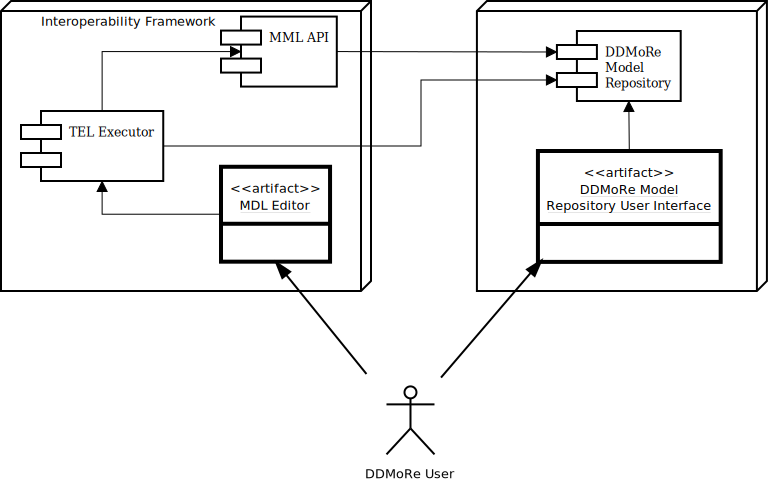
\includegraphics{img/UserInteraction}
\caption{Interactions between users, the interoperability framework and the Model Repository.}
\label{fig:userInteraction}
\end{figure}


%------------------------------------------------------------------------------
%Description       : DDMoRe WP7.2.1 Functional Specification for the Model
%                                   Repository Infrastructure - Requirements Survey 
%Authors           : Mihai Glonț <mglont@ebi.ac.uk>
%                    Camille Laibe <laibe@ebi.ac.uk>
%Organization      : EMBL-EBI
%                    Wellcome Trust Genome Campus
%                    Hinxton
%                    Cambridge
%                    United Kingdom
%------------------------------------------------------------------------------
\section{Requirements}
\label{requirements}
This section lists the needs, goals and constraints of the \ddmore Model Repository, grouped into two main categories: the former is dedicated to \glspl{functionalRequirement}, while the latter contains \glspl{nonFunctionalRequirement}. 

\subsection{Functional requirements}
\label{functionalRequirements}
%% Create a row counter so that we don't have to keep track of the ID of the functional requirement http://tex.stackexchange.com/questions/21243/automatic-table-row-numbers/21244#21244
%\newcounter{frCounter}
%\newcommand\frIndex{\stepcounter{frCounter}\arabic{frCounter}}

\begin{enumerate}[1]
\subsubsection{Model management}
\item The system is REQUIRED to store models encoded in \gls{MML}. Supplementary data files, processing scripts, textual and graphical representations of results, as well as reports SHOULD also be kept in the system. In addition, the concept of a project SHOULD be provided, grouping together related models. 

\item The system MUST allow appropriate users to store updated versions of models encoded in MML.

\item The system SHOULD maintain a record of the submissions of a given model to regulatory bodies including, but not limited to FDA, EMA, MHRA. The Repository SHOULD provide open access to the model's public assessment report or summary basis for approval if such reports exist. 

\item The system MUST be able to store relations and dependencies between different models.

\item The system MAY allow specific \glspl{revision} to be deleted by their owners, but no revision SHALL be lost from the Repository. In this case, users that had access to a model revision before its deletion SHALL continue to do so. The system SHOULD inform the user about the removal and MAY supply a link to a model revision which replaces it, if this information has been specified by the user that performed the deletion. 

\item Authenticated users SHOULD be able to subscribe to notifications about a model they have access to when it is updated.

\item The system MUST enable the creation of new models encoded in MML based on either an existing one, or a template. The system SHALL record for the new model a reference  to the representation from which it derives.

\item Models SHOULD be classified using descriptive and categorical tags, such as the ones done as part of WP4.

\item All versions of a given model MUST be preserved and be accessible.

\item The system SHALL ensure that in the event of concurrent modifications of the same model(s), neither set of changes is lost.

\item Models MAY be modified via an integrated editor.

\subsubsection{Model browsing, searching and retrieving}
\item The system MUST be able to search for the latest revision of model descriptions based on a textual term such as name, author, date of creation, date of modification, or any other textual field in MML. The results MUST only include models to which the user has access to. The system SHOULD also provide a configuration option that allows every version of every accessible model to be included in the model search.

% Topics are expressed using metadata. We already have requirements for including annotations in the search and for downloading a selection of models.
%\item The system MUST allow the retrieval of all models dealing with a certain topic. 

\item The system MAY allow a selection of search results, bundled as an archive, to be downloaded.

\item Users MAY be able to inspect differences between different versions of the same model.

\item The system MAY allow a selection of two models to be compared against a user-specified set of criteria.

\item Models and associated graphical representations stored as PNG or JPEG files MUST be displayed in an organised and user-friendly manner. This SHOULD include an export from the graphical viewer for MDL developed within Task 2.5.1, if such an export has been provided.

\item The inputs and outputs accompanying a model (included in the MML representation) MUST also be displayed along with an explanation. 

\item Users SHALL be able to retrieve and download any revision of any model they can access.

\item Model search SHOULD include model metadata such as annotations and tags.

\item The system SHOULD be able to search for models based on complex queries. Results SHOULD be ranked, for instance by using a combination of text retrieval, ontologies as well as model metadata as described in \cite{Henkel2010} and \cite{Schulz2011}. 

\subsubsection{Model quality}
\item The system is REQUIRED to check that model representations are faithful to the MML specification either on-demand -- upon request, or autonomously -- whenever the need arises, such as before accepting a new revision for a model. 

\item The system MUST accommodate a system of reviews and more informal comments. The presence of reviews could be used as a criterion for comparing models.

\item The system MAY indicate whether a model runs successfully or not on. If this feature is implemented, the system SHOULD NOT allow a model to be reviewed or published unless it can be simulated locally. 

\subsubsection{Authentication and authorisation}
\item The system MUST authenticate users and ensure that they can only perform the role assigned to them for a given model (cf. Section~\ref{users}).

\item The Repository MUST maintain a model \gls{audit trail}, storing each revision with additional information about its content including, but not limited to the identity of the user performing the action and a timestamp. Users MAY add a comment describing the changes they introduce. The level of detail of this information SHOULD be configurable at the level of the instance by an Administrator. 

\item The level of visibility of the audit information associated with a published model SHOULD be configurable at the level of the instance by an Administrator.

\item For the safety and integrity of the Repository, a system-wide audit trail, that MUST only be available to Administrators, MUST record security-relevant events including but not limited to changes to model data, metadata, ownership, or access rights. 

\item A model owner MUST be allowed to grant read and write access to a model using one of the following options:
\begin{inparaenum}
\item a single revision 
\item all existing revisions 
\item all revisions including the ones in the future. 
\end{inparaenum} 

\item Once granted, read rights to a revision for a particular user SHALL NOT be revoked: once users have gained read access to a model, they might have already collected all relevant information.

\item The system MUST enable model owners to revoke write access to future revisions of a model for a single user or group of users simultaneously.

\item The system MUST enable model owners to publish a single version of a model. This action SHALL not impact the status of previous model revisions. 

\item The Owner SHOULD be able to grant write access to an unpublished model to a single user, or to a group of users. This would allow Editors to upload new model revisions. The system is then REQUIRED to automatically grant read and write access to a revision for the Editor who uploaded it.

\item A model owner SHOULD be allowed to transfer the complete ownership of a model to another existing user.

\item The owner SHOULD be able to control the access rights of other users to read or write the model.

\item Unauthenticated access to the published models in the system SHOULD be permitted as a configuration option. If this option is disabled, users MUST be authenticated before they can access any models within the system.

\item The system MUST be protected against SQL injection, cross-site scripting as well as cross-site request forgery attacks. 

\subsubsection{Interaction with the Interoperability Framework}
\item Programmatic access to models within the Repository MUST be provided to other software systems including, but not limited to those within \ddmore. In particular, the interoperability platform developed within WP2 MUST be able to load models from the system. This SHOULD be accomplished by means of web services and/or messaging queues. 

\item The system MAY enable a user to launch the simulation of a model with their own data sets using their local Infrastructure. 

\subsubsection{Technology}
\item The system SHALL store models represented in MML format.

\item The server side of the system is REQUIRED to work on a GNU Linux platform with kernel version~$\ge 2.6$. 

\item The client side SHALL work with the following operating systems: Mac OS X (Leopard, Version 10.5.x and newer versions), Windows (Windows XP and newer versions), GNU Linux (kernel version~$\ge 2.6$).

\item The client side MUST work with the following web browsers: Safari Version 5.x and above, Internet Explorer 8 and above, Firefox Version 10.x and above. The front end MAY work in other browsers.

\item An established software version control system such as Subversion, Mercurial or Git MAY be used by the system internally, however, it MUST NOT be exposed to users directly.

%% user management requirements are missing from the original document
\subsubsection{User management}
\item An administrator MUST be able to manage user accounts. This covers creation, suspension, deletion, blocking or unblocking.

\item The system MUST allow an authenticated user or administrator to update certain details of an account including but not limited to password, name, contact details. Due care MUST be taken to ensure that the user confirms their identity before editing this information.
\end{enumerate}

\subsection{Non-functional requirements}
\label{nonFunctionalRequirements}
\begin{enumerate}[1]
\setcounter{enumi}{50}
% TODO: should we actually put that?
%\item The system MUST be responsive, completing 80\% of requests in under 10 seconds and 95\% of requests in under 30 seconds on a computer with 2GB RAM, dual-core processor and 1Mb/s Internet connection.

\item The user interface of the system SHALL be designed with usability in mind, displaying information in a meaningful and user-friendly manner to its stakeholders, without overloading them.

\item The system MUST provide meaningful user information in case of an error. If the error is caused by the system (rather than the user), the system MUST log all necessary information in order to allow a fix to be developed.

\item The look and feel of the Repository MUST be configurable by means of skins.

\item The system SHALL notify users when a request cannot be processed immediately, either by indicating the progress or by notifying the user when the process has been completed.

\item The system SHALL be implemented using modern presentation and accessibility standards in order to aid maintainability.

\item The system SHOULD be installable and configurable as a software distribution.

\item The system SHOULD be modular and allow extension.
\end{enumerate}


%------------------------------------------------------------------------------
%Description       : DDMoRe WP7.2.1 First Technical Specification for the Model
%                                   Repository Infrastructure - Proposed Design 
%Author            : Mihai Glonț <mglont@ebi.ac.uk>
%Organization      : EMBL-EBI
%                    Wellcome Trust Genome Campus
%                    Hinxton
%                    Cambridge
%                    United Kingdom
%------------------------------------------------------------------------------
\section{Proposed Design}
\label{proposedDesign}
\idea{Add general description of the topics covered in this section.}

\subsection{Use Cases}
\label{useCases}
The aim of this section is to describe how each of the aforementioned stakeholders interact with the system. Each such interaction is called a \gls{usecase}, while the user performing it is known as an \gls{actor}. The use cases listed in Figure~\ref{fig:useCases} only consider the main actors that are involved, hence Administrators are not mentioned in any model-related use cases, in spite of the fact that they do have the authority required to perform any action. 

\begin{figure}[htb]
\centering
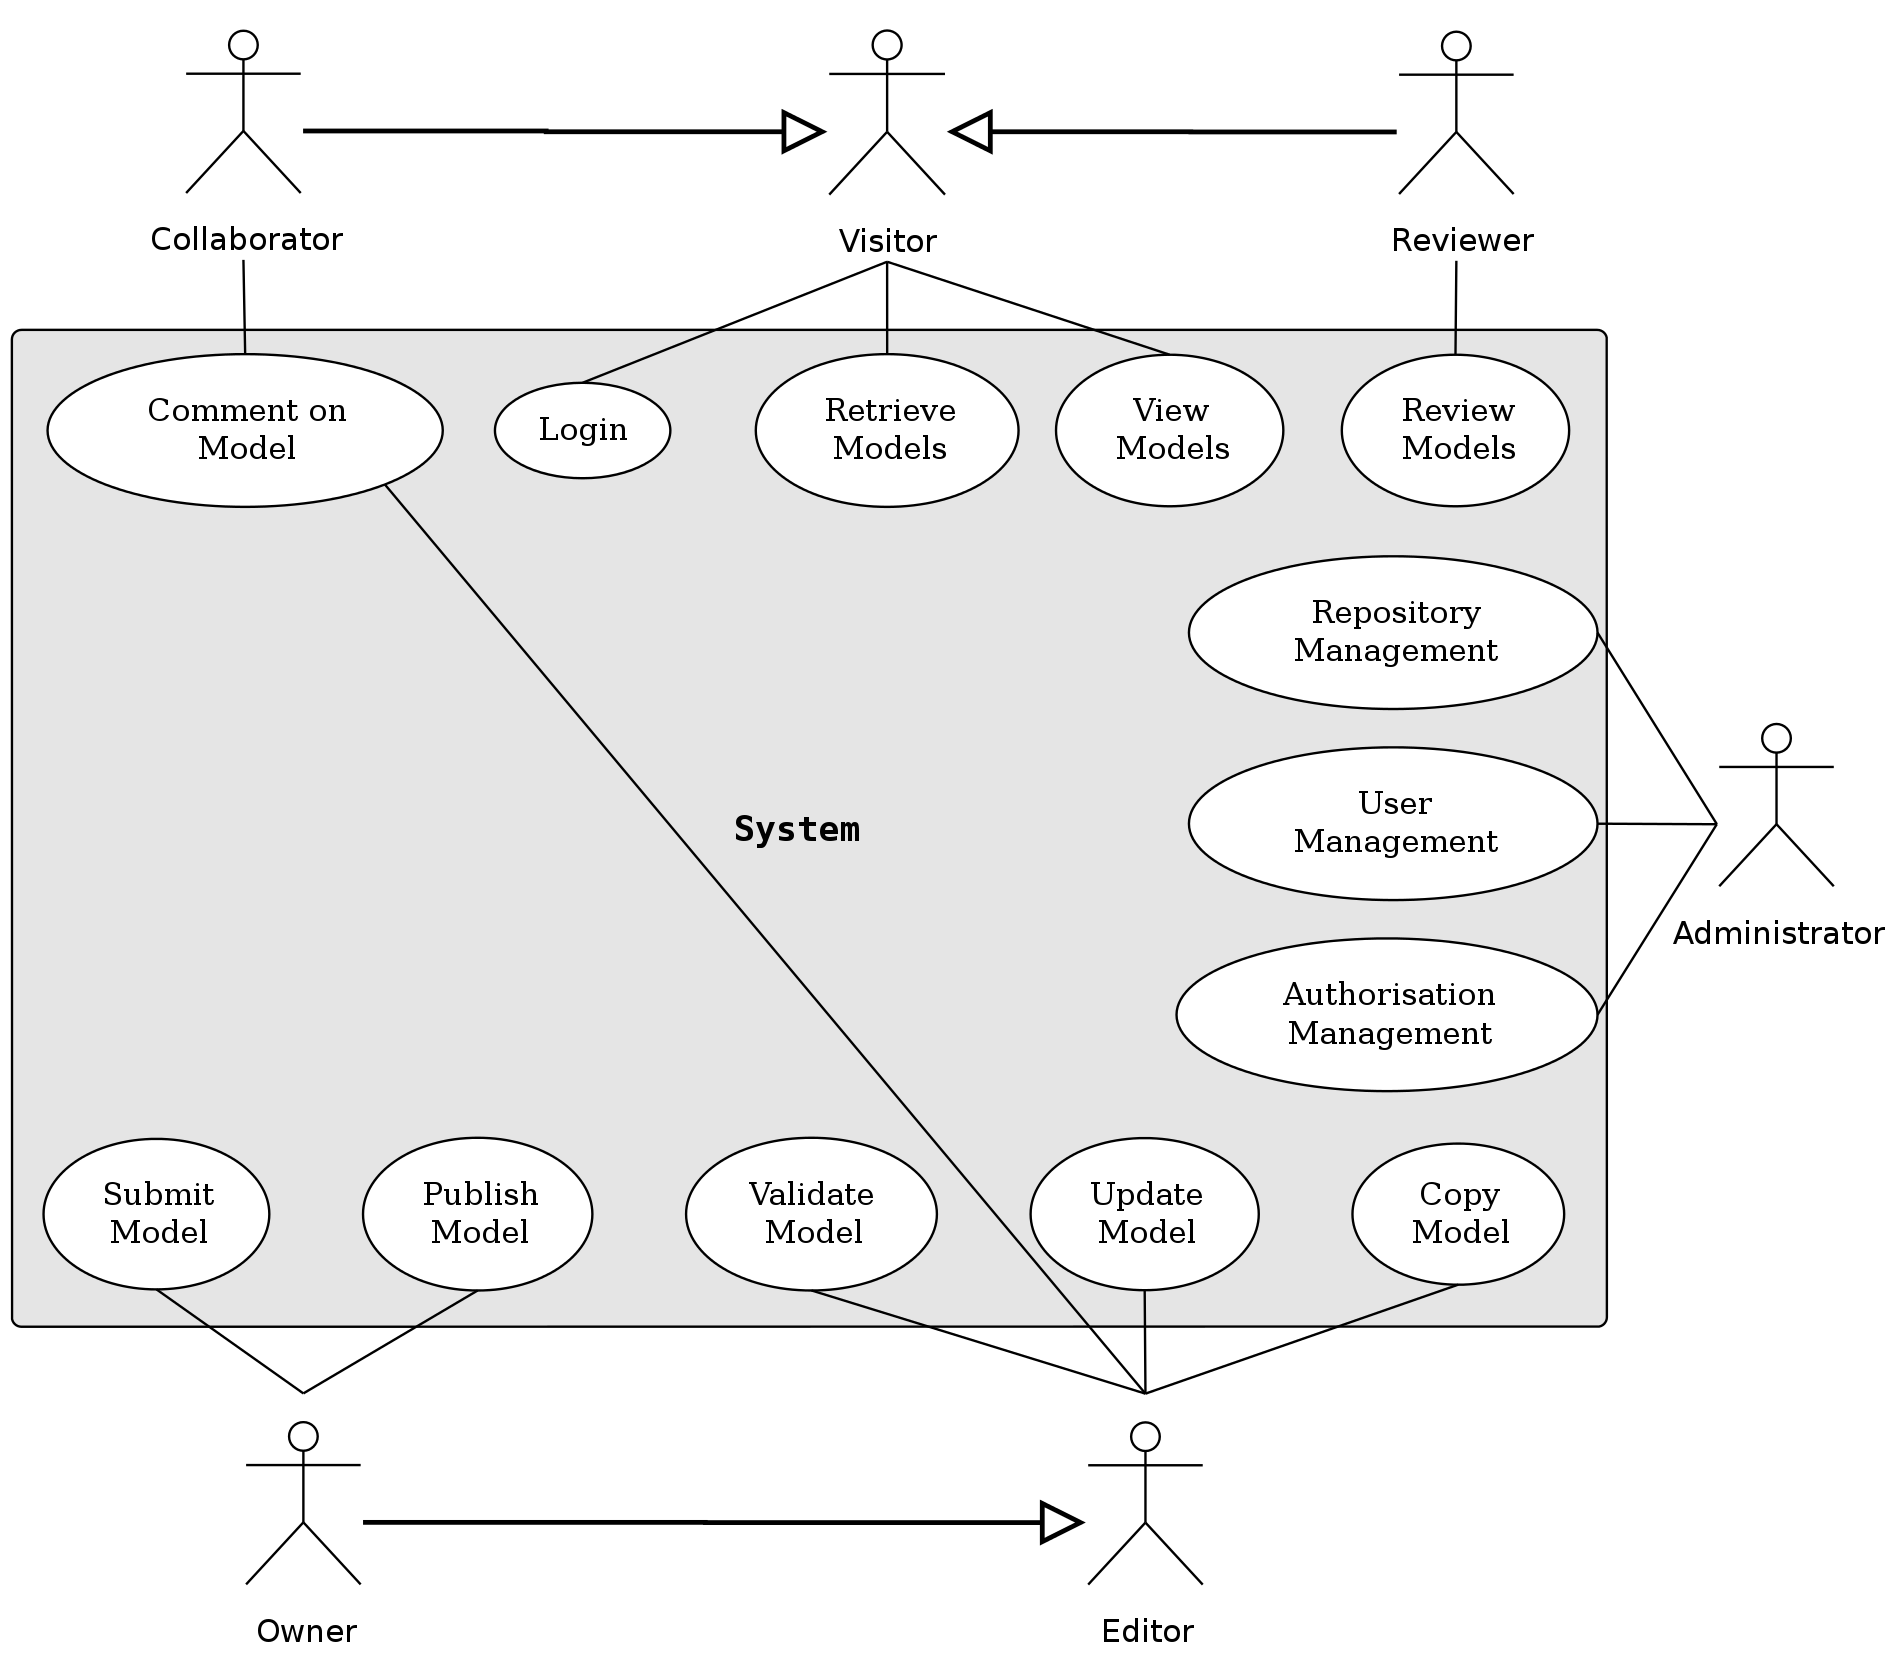
\includegraphics{img/UseCases}
\caption{Diagrammatic representation of the system's scope.}
\label{fig:useCases}
\end{figure}

\subsection{Proposed Work flows}
\label{workFlows}
\idea{UML Activity and Sequence diagrams should go in the appendix, should there be many of them. This section should only discuss them.} 

\subsection{Software Infrastructure}
\label{softwareInfrastructure}
\idea{Add UML Deployment diagram showing the link between a DB server, a Web server (possibly a servlet container behind an HTTP server) and a folder under version control.}

\subsection{Mock-ups}
\label{mockUps}
\idea{General UXD comments behind the look and feel of the pages. Actual mock-ups should be in the appendix. Landscape page format might be required for this part.}

\input{webServices}

\subsection{Security Considerations}
\label{securityConsiderations}
\idea{Exclude data centre, hardware and network security aspects from the scope of this document. Recommend running the HTTP server and the servlet container as different users with limited privileges. Beware that the user running the servlet container needs write access to the folder storing models. Discuss the need to protect the metadata directory within the folder where the models are stored (e.g. .git, .hg, .svn), as access to them outside the designated protocol - i.e. the web interface - should be prohibited.}

\subsection{Licence}
\label{licence}
The code for the \ddmore Model Repository will be hosted on SourceForge and released under a GPL-compatible licence. This licence does not apply to the models stored in either the public Repository or any private instance of it. 


%------------------------------------------------------------------------------
%Description       : DDMoRe WP7.2.1 First Technical Specification for the Model
%                                   Repository Infrastructure - Web Services
%Author            : Mihai Glonț <mglont@ebi.ac.uk>
%Organization      : EMBL-EBI
%                    Wellcome Trust Genome Campus
%                    Hinxton
%                    Cambridge
%                    United Kingdom
%------------------------------------------------------------------------------
\subsection{Programmatic Interaction with the \ddmore Model Repository}
\label{webServices}
\idea{This section is dedicated to programmatic access to and manipulation of models. It should provide a diagrammatic representation of the envisaged architecture along with the considerations behind it. A discussion on the integration with other software systems within \ddmore should also be included.}



\section{Final Considerations} 

\subsection{Software Infrastructure}
\label{softwareInfrastructure}
The \ddmore Model Repository stores models under version control on the file system, while the metadata associated with them is maintained in a relational database. Consequently, an instance of the Repository may be deployed along with a database server and a web server communicating over LAN. The models within the Repository should be contained in a centralised location which should be accessible from the web server.

\subsection{Security Considerations}
\label{securityConsiderations}
\idea{Exclude data centre, hardware and network security aspects from the scope of this document. Recommend running the HTTP server and the servlet container as different users with limited privileges. Beware that the user running the servlet container needs write access to the folder storing models. Discuss the need to protect the metadata directory within the folder where the models are stored (e.g. .git, .hg, .svn), as access to them outside the designated protocol - i.e. the web interface - should be prohibited.}

\subsection{Licence}
\label{licence}
The code for the \ddmore Model Repository will be hosted on SourceForge and released under a GPL-compatible licence. This licence does not apply to the models stored in either the public Repository or any private instance of it. 


%\begin{landscape}
\section{Appendices}
\label{appendices}
\subsection{Mock-up Designs}
\label{appendix1}

\begin{figure}[htb]
	\centering
	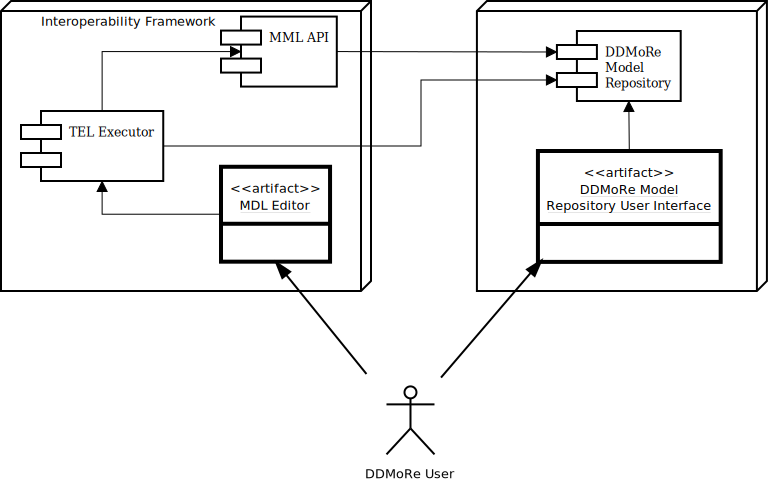
\includegraphics[width=0.75\linewidth]{img/UserInteraction}
	\caption{Overview of the interaction between \ddmore users and the Model Repository.}
	\label{fig:userInteraction1}
\end{figure}
\end{landscape}
\clearpage

\subsection{UML Activity Diagrams}
\label{appendix2}
\clearpage

\clearpage
%% Display the full name of authors and sort by author
\bibliographystyle{unsrt}
\bibliography{technical-specification}
\end{document}


%% Change the style of the glossary terms
\renewcommand{\glsnamefont}[1]{\textit{#1}}

\newcommand{\ddmore}{DDMoRe\xspace}

\newcommand{\idea}[1]{\fbox{\parbox{0.98\linewidth}{\emph{#1}}}}

%\newcommand{\techNote}[1]{\vspace{1em} \fbox{\parbox{\linewidth}{{\Large \color{techNoteTitle} \textit{Technical Note}}\\ \textrm{\color{techNoteText} #1}}} \vspace{1em}} 

\definecolor{tnTitle}{HTML}{BF0069}
\definecolor{tnBox}{HTML}{EDE800}
\definecolor{tnBody}{HTML}{065B98}

\newenvironment{techNote}
  {\vspace{1em}\par\begin{mdframed}[linewidth=2pt,linecolor=tnBox]%
  	{\textcolor{tnTitle}{\Large \emph{Technical Note}}}%
    \begin{list}{}{\leftmargin=1em
                   \labelwidth=\leftmargin \color{tnBody}}\item[\Large\ding{43}]} 
  {\end{list}\end{mdframed}\par \vspace{1em}}


\makeglossaries

\begin{document}
%------------------------------------------------------------------------------
%Description       : DDMoRe WP7.2.1 Functional Specification for the Model
%                                   Repository Infrastructure - title 
%Author            : Mihai Glonț <mglont@ebi.ac.uk>
%Organization      : EMBL-EBI
%                    Wellcome Trust Genome Campus
%                    Hinxton
%                    Cambridge
%                    United Kingdom
%------------------------------------------------------------------------------
%% Don't insert a break after the title page.
\let\endtitlepage\relax

\fancypagestyle{firstpage}
{
    \fancyhf{}
    \fancyhead[R]{
\includegraphics[scale=0.5]{img/ddmore_logo}}
}

\begin{titlepage}
\thispagestyle{firstpage}
\begin{center}
{\huge Functional Specification of the \ddmore Repository Infrastructure}\\[15pt]

{\LARGE WP7 Sub-Task 7.2.1}\\[10pt]

Camille Laibe
\qquad Mihai Glon\textcommabelow{t}
\\[5pt]

\textsc{{\footnotesize EMBL-EBI, Wellcome Trust Genome Campus, Cambridge, United Kingdom}}
\end{center}
\end{titlepage}



\section*{Document revision history}
\begin{tabularx}{\linewidth}{c c X}\hline
\textit{Date} & \textit{Author} & \textit{Comments} \\ \hline
1 August & Mihai Glon\cb{t} & First draft \\ 
5 September & Camille Laibe & First set of corrections and additions \\ 
7 September & Mihai Glon\cb{t} & Incorporated comments from Jonathan Chard \\ 
20 September & Mihai Glon\cb{t} & Incorporated comments from Lutz Harnisch, Alain Munafo and Paolo Magni \\ 
31 October & Mihai Glon\cb{t} & Extensively revised the structure and the language employed to aid understanding. \\ \hline
\end{tabularx}


\section*{Disclaimer} 
This document is under development. When deemed fit for release, it will be published in the deliverables section for WP7. It will continue to be subject to incremental updates whenever the need arises. 


\section*{Terms of use}
This document is distributed under the Creative Commons Attribution-ShareAlike (CC BY-SA) License~\cite{CC-SA}. 


\section*{Conventions}
The key words "MUST", "MUST NOT", "REQUIRED", "SHALL", "SHALL NOT", "SHOULD", "SHOULD NOT", "RECOMMENDED",  "MAY", and "OPTIONAL" in this document are to be interpreted as described in RFC 2119\cite{RFC2119}.

Throughout this document the term \emph{Model Repository} has been preferred over \emph{Model Library} (used in the Description of Work~\cite{ddmore:dow}) for better clarity and to avoid misunderstandings. It denotes the technical infrastructure required to store model descriptions, along with data, metadata and cross-references.


\section*{Acknowledgements}
 We are grateful to Stuart Moodie, Maciej Swat and  Nicolas Le~Nov{\`e}re for their involvement in capturing the needs of the Repository~\cite{mli:req}, which was the starting point for this document.

\clearpage
\pagenumbering{roman}
\setcounter{page}{1}
\tableofcontents
\listoffigures
\clearpage

\printglossaries
\clearpage

%% Each file contains a separate section to aid collaboration.
\pagenumbering{arabic}
%------------------------------------------------------------------------------
%Description       : DDMoRe WP7.2.1 First Technical Specification for the Model
%                                   Repository Infrastructure - Introduction 
%Authors           : Mihai Glonț <mglont@ebi.ac.uk>
%                    Camille Laibe <laibe@ebi.ac.uk>
%Organization      : EMBL-EBI
%                    Wellcome Trust Genome Campus
%                    Hinxton
%                    Cambridge
%                    United Kingdom
%------------------------------------------------------------------------------
\section{Introduction}
\label{introduction}
This document provides a detailed description of the functionality that will be provided by the \ddmore Model Repository. The guidelines herein apply not only to the public Repository, but also to any private instances of it.

\subsection{Scope}
This document reviews the characteristics of the \ddmore Model Repository in relation to the wider context of the project, outlining along the way envisaged workflows, interactions with both users and third party software, as well as potential software dependencies of the Repository. The intended audience for this specification are the EFPIA and academic partners that wish to use the Repository in an optimal manner, or are merely interested in its capabilities.

\subsection{Non-Goals}
Although this task should deliver a technical specification at this stage according to the Description of Work, it is paramount that the behaviour of the Repository meets the needs of its end-users. Therefore, this document aims to offer a mental picture of the features that have been incorporated into the design of the Repository, allowing the interested stakeholders to flag up any shortcomings. Implementation-specific details about the inner-workings of the Repository are outside of the scope of this document, but will be discussed in the second technical specification which is due in month 42 of the project. 

\subsection{Context}
\label{context}
In a world where inefficient data and knowledge-sharing between academia, pharmaceutical companies and regulatory bodies hinders the development of better medicines, the Drug Disease Model Resources project (\ddmore) -- a Europe-wide effort funded by Innovative Medicines Initiative Joint Undertaking -- seeks to create an environment governed by standards that addresses these shortcomings. Specifically, the \ddmore consortium is developing a common definition language for data, models and work flows, as well as a standard for storing and exchanging \glspl{model} and associated \gls{metadata}\cite{ddmore:dow}.

The main focus on this specification is the objective of Task 7.2: the \ddmore Model Repository. It aims to provide a central repository for the models created by the project, encouraging their reuse. The Repository is closely linked with other deliverables of \ddmore. For instance, the pre-competitive models that will populate the Model Repository initially will be provided by Work Package 1. The models will be encoded in the XML-based format developed by WP4, and the Repository will rely on the software library created by Task 2.3 in order to manipulate the models. Finally, the published models stored in the \ddmore Model Repository will be showcased in the public instance of the Modelling Framework, generated by Task 7.1.

\subsection{Objectives}
\label{objectives}
The main objectives of the Repository are to provide:
\begin{itemize}
  \item a central, versioned, storage place for public and private models
  \item a way to display individual models
  \item a way to search for models
  \item a way to download models
  \item various means to access the stored \glspl{model}, making available the information encoded in MML to both users and tools. 
\end{itemize}

\subsection{Type of users}
\label{users}
This section classifies the users of the \ddmore Model Repository into categories. With the exception of Administrators, whose permissions are granted at global level, over the entire instance of the Repository, all other roles that require authentication are defined at the level of a specific revision. This means that the owner of one model can also be the editor of a revision for another model. 

\begin{description}
  \item[Visitor] an anonymous user accessing \glspl{published model}.
  \item[Owner] the user who submitted the model and has ultimate ownership of what is done to it and how and
when it is published.
  \item[Editor] any user who is able to modify and add information to an existing published or \gls{unpublished model}. Typically the Owner of a model is also an Editor of this model.
  \item[Collaborator] any user who is able to access an unpublished model.
  \item[Reviewer] a user who can access an unpublished model. This role can be limited in time.
  \item[Administrator] a user who is responsible for the security, management and maintenance of the system.
\end{description}

The interactions between users, the Model Repository and other components of the project (such as the Interoperability Framework) are depicted in Figure~\ref{fig:userInteraction}. As such, one may access the Repository directly -- through the web-based user interface -- or indirectly, via the Modelling Interoperability Framework, that uses the Task Execution Language (TEL) and the software library created in WP2.3 to access and store models in the \ddmore Model Repository.

\begin{figure}[htb]
\centering
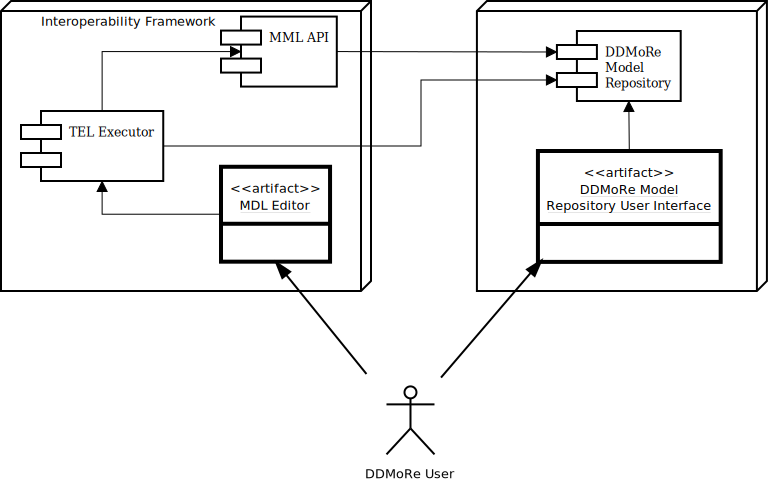
\includegraphics{img/UserInteraction}
\caption{Interactions between users, the interoperability framework and the Model Repository.}
\label{fig:userInteraction}
\end{figure}


%------------------------------------------------------------------------------
%Description       : DDMoRe WP7.2.1 Functional Specification for the Model
%                                   Repository Infrastructure - Requirements Survey 
%Authors           : Mihai Glonț <mglont@ebi.ac.uk>
%                    Camille Laibe <laibe@ebi.ac.uk>
%Organization      : EMBL-EBI
%                    Wellcome Trust Genome Campus
%                    Hinxton
%                    Cambridge
%                    United Kingdom
%------------------------------------------------------------------------------
\section{Requirements}
\label{requirements}
This section lists the needs, goals and constraints of the \ddmore Model Repository, grouped into two main categories: the former is dedicated to \glspl{functionalRequirement}, while the latter contains \glspl{nonFunctionalRequirement}. 

\subsection{Functional requirements}
\label{functionalRequirements}
%% Create a row counter so that we don't have to keep track of the ID of the functional requirement http://tex.stackexchange.com/questions/21243/automatic-table-row-numbers/21244#21244
%\newcounter{frCounter}
%\newcommand\frIndex{\stepcounter{frCounter}\arabic{frCounter}}

\begin{enumerate}[1]
\subsubsection{Model management}
\item The system is REQUIRED to store models encoded in \gls{MML}. Supplementary data files, processing scripts, textual and graphical representations of results, as well as reports SHOULD also be kept in the system. In addition, the concept of a project SHOULD be provided, grouping together related models. 

\item The system MUST allow appropriate users to store updated versions of models encoded in MML.

\item The system SHOULD maintain a record of the submissions of a given model to regulatory bodies including, but not limited to FDA, EMA, MHRA. The Repository SHOULD provide open access to the model's public assessment report or summary basis for approval if such reports exist. 

\item The system MUST be able to store relations and dependencies between different models.

\item The system MAY allow specific \glspl{revision} to be deleted by their owners, but no revision SHALL be lost from the Repository. In this case, users that had access to a model revision before its deletion SHALL continue to do so. The system SHOULD inform the user about the removal and MAY supply a link to a model revision which replaces it, if this information has been specified by the user that performed the deletion. 

\item Authenticated users SHOULD be able to subscribe to notifications about a model they have access to when it is updated.

\item The system MUST enable the creation of new models encoded in MML based on either an existing one, or a template. The system SHALL record for the new model a reference  to the representation from which it derives.

\item Models SHOULD be classified using descriptive and categorical tags, such as the ones done as part of WP4.

\item All versions of a given model MUST be preserved and be accessible.

\item The system SHALL ensure that in the event of concurrent modifications of the same model(s), neither set of changes is lost.

\item Models MAY be modified via an integrated editor.

\subsubsection{Model browsing, searching and retrieving}
\item The system MUST be able to search for the latest revision of model descriptions based on a textual term such as name, author, date of creation, date of modification, or any other textual field in MML. The results MUST only include models to which the user has access to. The system SHOULD also provide a configuration option that allows every version of every accessible model to be included in the model search.

% Topics are expressed using metadata. We already have requirements for including annotations in the search and for downloading a selection of models.
%\item The system MUST allow the retrieval of all models dealing with a certain topic. 

\item The system MAY allow a selection of search results, bundled as an archive, to be downloaded.

\item Users MAY be able to inspect differences between different versions of the same model.

\item The system MAY allow a selection of two models to be compared against a user-specified set of criteria.

\item Models and associated graphical representations stored as PNG or JPEG files MUST be displayed in an organised and user-friendly manner. This SHOULD include an export from the graphical viewer for MDL developed within Task 2.5.1, if such an export has been provided.

\item The inputs and outputs accompanying a model (included in the MML representation) MUST also be displayed along with an explanation. 

\item Users SHALL be able to retrieve and download any revision of any model they can access.

\item Model search SHOULD include model metadata such as annotations and tags.

\item The system SHOULD be able to search for models based on complex queries. Results SHOULD be ranked, for instance by using a combination of text retrieval, ontologies as well as model metadata as described in \cite{Henkel2010} and \cite{Schulz2011}. 

\subsubsection{Model quality}
\item The system is REQUIRED to check that model representations are faithful to the MML specification either on-demand -- upon request, or autonomously -- whenever the need arises, such as before accepting a new revision for a model. 

\item The system MUST accommodate a system of reviews and more informal comments. The presence of reviews could be used as a criterion for comparing models.

\item The system MAY indicate whether a model runs successfully or not on. If this feature is implemented, the system SHOULD NOT allow a model to be reviewed or published unless it can be simulated locally. 

\subsubsection{Authentication and authorisation}
\item The system MUST authenticate users and ensure that they can only perform the role assigned to them for a given model (cf. Section~\ref{users}).

\item The Repository MUST maintain a model \gls{audit trail}, storing each revision with additional information about its content including, but not limited to the identity of the user performing the action and a timestamp. Users MAY add a comment describing the changes they introduce. The level of detail of this information SHOULD be configurable at the level of the instance by an Administrator. 

\item The level of visibility of the audit information associated with a published model SHOULD be configurable at the level of the instance by an Administrator.

\item For the safety and integrity of the Repository, a system-wide audit trail, that MUST only be available to Administrators, MUST record security-relevant events including but not limited to changes to model data, metadata, ownership, or access rights. 

\item A model owner MUST be allowed to grant read and write access to a model using one of the following options:
\begin{inparaenum}
\item a single revision 
\item all existing revisions 
\item all revisions including the ones in the future. 
\end{inparaenum} 

\item Once granted, read rights to a revision for a particular user SHALL NOT be revoked: once users have gained read access to a model, they might have already collected all relevant information.

\item The system MUST enable model owners to revoke write access to future revisions of a model for a single user or group of users simultaneously.

\item The system MUST enable model owners to publish a single version of a model. This action SHALL not impact the status of previous model revisions. 

\item The Owner SHOULD be able to grant write access to an unpublished model to a single user, or to a group of users. This would allow Editors to upload new model revisions. The system is then REQUIRED to automatically grant read and write access to a revision for the Editor who uploaded it.

\item A model owner SHOULD be allowed to transfer the complete ownership of a model to another existing user.

\item The owner SHOULD be able to control the access rights of other users to read or write the model.

\item Unauthenticated access to the published models in the system SHOULD be permitted as a configuration option. If this option is disabled, users MUST be authenticated before they can access any models within the system.

\item The system MUST be protected against SQL injection, cross-site scripting as well as cross-site request forgery attacks. 

\subsubsection{Interaction with the Interoperability Framework}
\item Programmatic access to models within the Repository MUST be provided to other software systems including, but not limited to those within \ddmore. In particular, the interoperability platform developed within WP2 MUST be able to load models from the system. This SHOULD be accomplished by means of web services and/or messaging queues. 

\item The system MAY enable a user to launch the simulation of a model with their own data sets using their local Infrastructure. 

\subsubsection{Technology}
\item The system SHALL store models represented in MML format.

\item The server side of the system is REQUIRED to work on a GNU Linux platform with kernel version~$\ge 2.6$. 

\item The client side SHALL work with the following operating systems: Mac OS X (Leopard, Version 10.5.x and newer versions), Windows (Windows XP and newer versions), GNU Linux (kernel version~$\ge 2.6$).

\item The client side MUST work with the following web browsers: Safari Version 5.x and above, Internet Explorer 8 and above, Firefox Version 10.x and above. The front end MAY work in other browsers.

\item An established software version control system such as Subversion, Mercurial or Git MAY be used by the system internally, however, it MUST NOT be exposed to users directly.

%% user management requirements are missing from the original document
\subsubsection{User management}
\item An administrator MUST be able to manage user accounts. This covers creation, suspension, deletion, blocking or unblocking.

\item The system MUST allow an authenticated user or administrator to update certain details of an account including but not limited to password, name, contact details. Due care MUST be taken to ensure that the user confirms their identity before editing this information.
\end{enumerate}

\subsection{Non-functional requirements}
\label{nonFunctionalRequirements}
\begin{enumerate}[1]
\setcounter{enumi}{50}
% TODO: should we actually put that?
%\item The system MUST be responsive, completing 80\% of requests in under 10 seconds and 95\% of requests in under 30 seconds on a computer with 2GB RAM, dual-core processor and 1Mb/s Internet connection.

\item The user interface of the system SHALL be designed with usability in mind, displaying information in a meaningful and user-friendly manner to its stakeholders, without overloading them.

\item The system MUST provide meaningful user information in case of an error. If the error is caused by the system (rather than the user), the system MUST log all necessary information in order to allow a fix to be developed.

\item The look and feel of the Repository MUST be configurable by means of skins.

\item The system SHALL notify users when a request cannot be processed immediately, either by indicating the progress or by notifying the user when the process has been completed.

\item The system SHALL be implemented using modern presentation and accessibility standards in order to aid maintainability.

\item The system SHOULD be installable and configurable as a software distribution.

\item The system SHOULD be modular and allow extension.
\end{enumerate}


%------------------------------------------------------------------------------
%Description       : DDMoRe WP7.2.1 First Technical Specification for the Model
%                                   Repository Infrastructure - Proposed Design 
%Author            : Mihai Glonț <mglont@ebi.ac.uk>
%Organization      : EMBL-EBI
%                    Wellcome Trust Genome Campus
%                    Hinxton
%                    Cambridge
%                    United Kingdom
%------------------------------------------------------------------------------
\section{Proposed Design}
\label{proposedDesign}
\idea{Add general description of the topics covered in this section.}

\subsection{Use Cases}
\label{useCases}
The aim of this section is to describe how each of the aforementioned stakeholders interact with the system. Each such interaction is called a \gls{usecase}, while the user performing it is known as an \gls{actor}. The use cases listed in Figure~\ref{fig:useCases} only consider the main actors that are involved, hence Administrators are not mentioned in any model-related use cases, in spite of the fact that they do have the authority required to perform any action. 

\begin{figure}[htb]
\centering
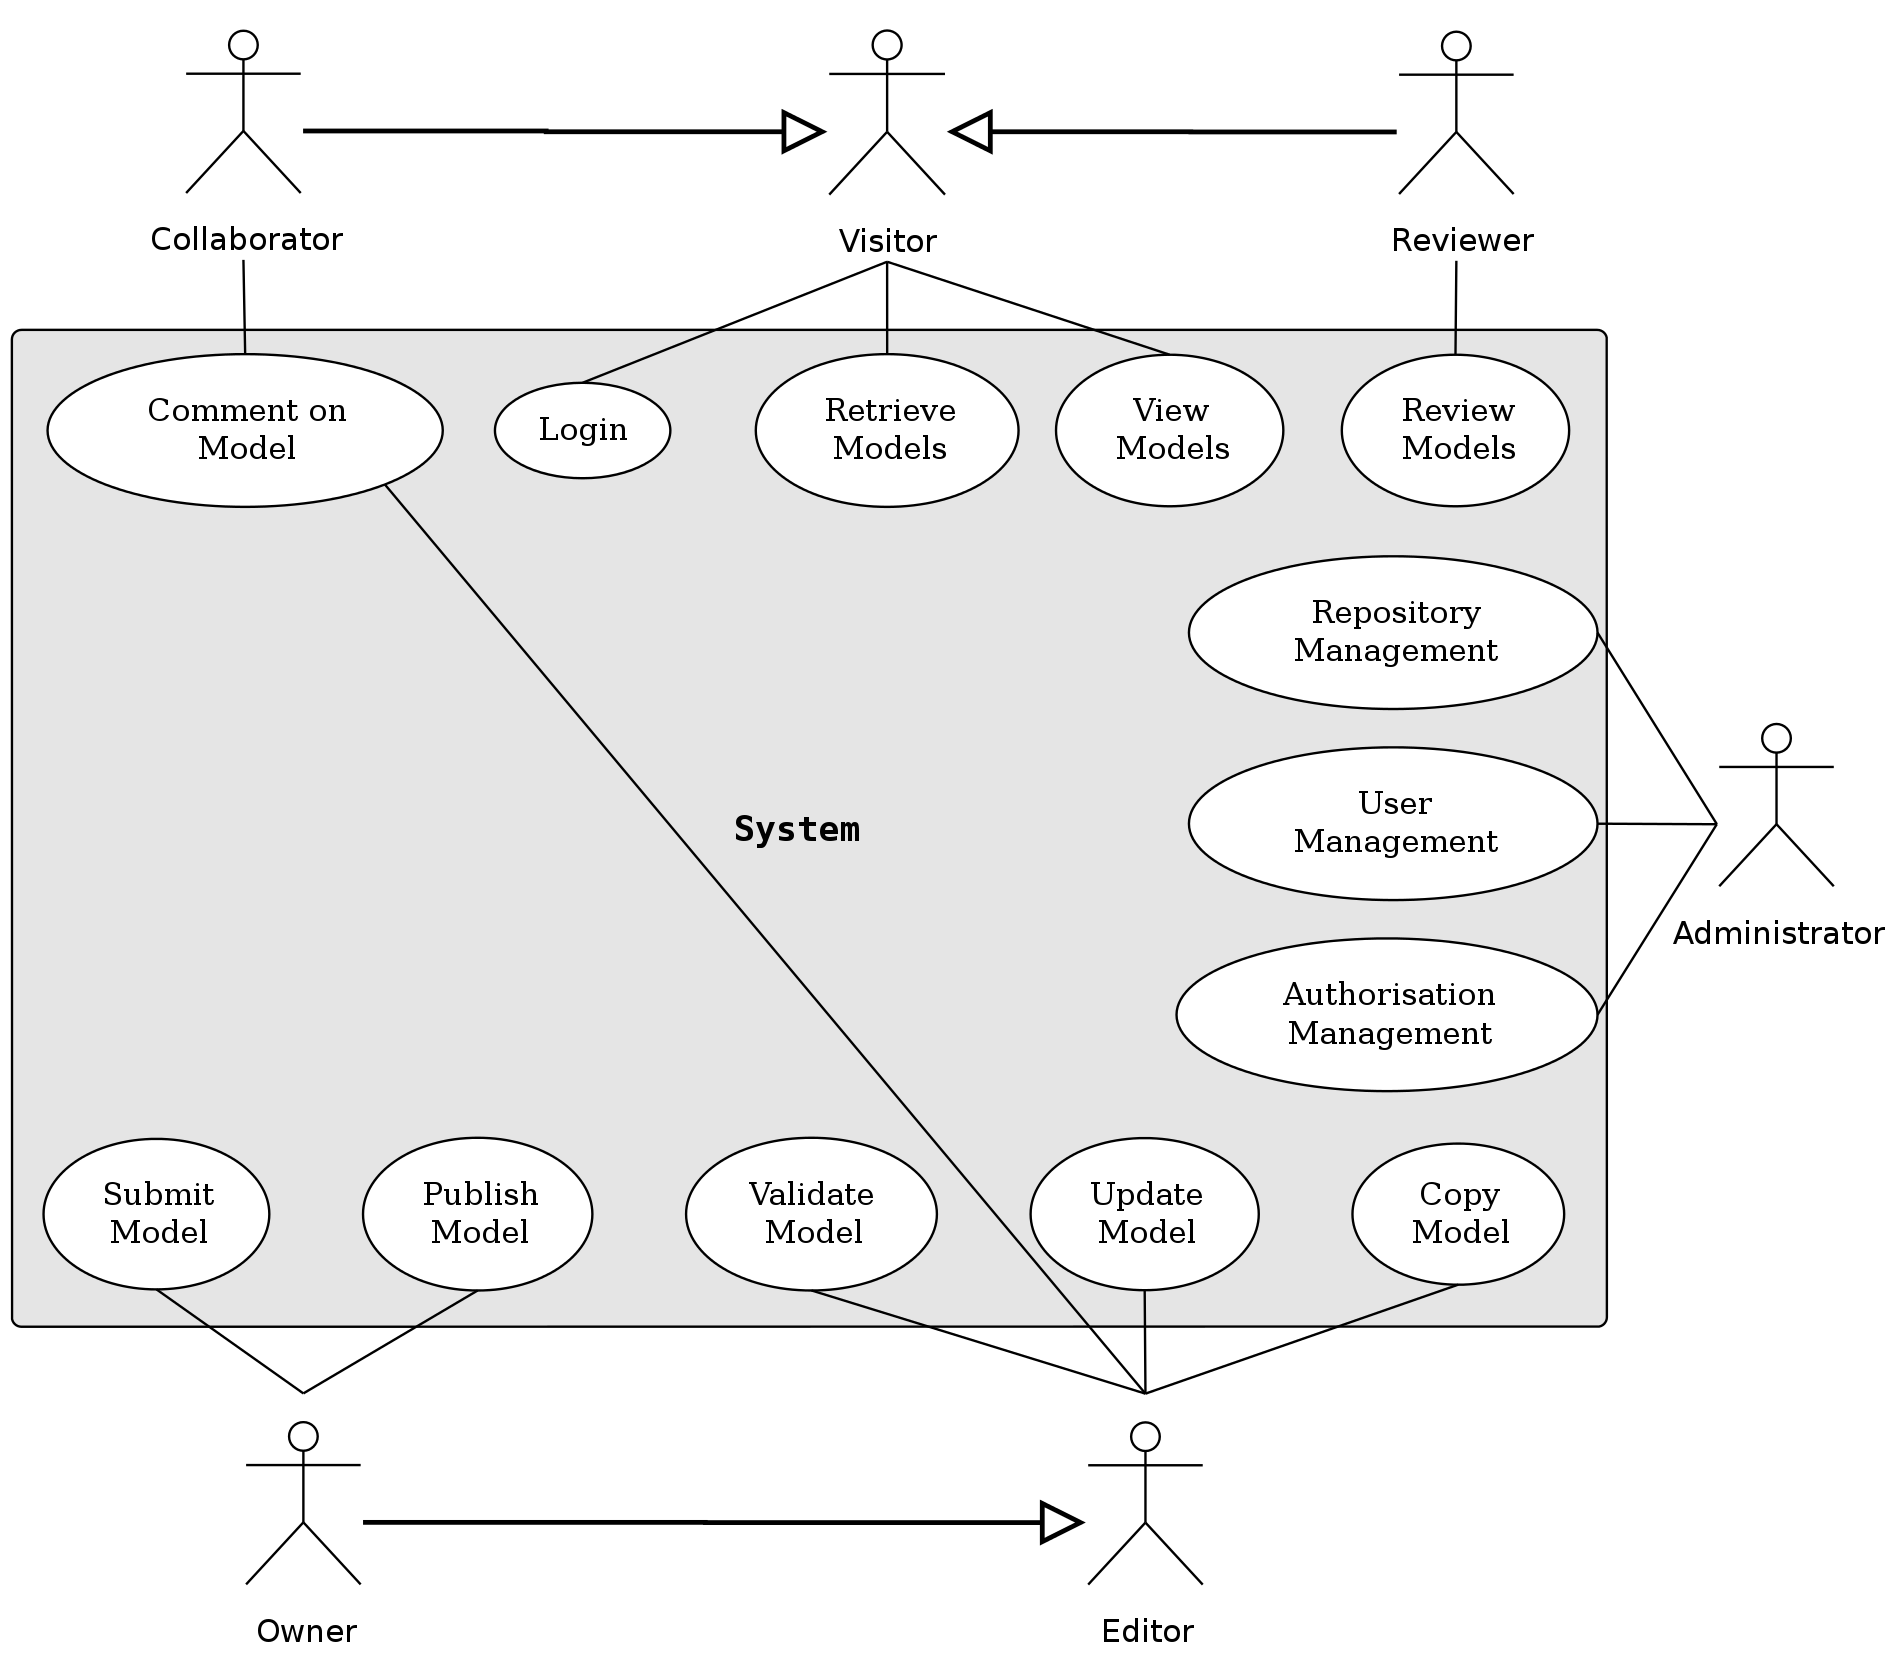
\includegraphics{img/UseCases}
\caption{Diagrammatic representation of the system's scope.}
\label{fig:useCases}
\end{figure}

\subsection{Proposed Work flows}
\label{workFlows}
\idea{UML Activity and Sequence diagrams should go in the appendix, should there be many of them. This section should only discuss them.} 

\subsection{Software Infrastructure}
\label{softwareInfrastructure}
\idea{Add UML Deployment diagram showing the link between a DB server, a Web server (possibly a servlet container behind an HTTP server) and a folder under version control.}

\subsection{Mock-ups}
\label{mockUps}
\idea{General UXD comments behind the look and feel of the pages. Actual mock-ups should be in the appendix. Landscape page format might be required for this part.}

%------------------------------------------------------------------------------
%Description       : DDMoRe WP7.2.1 First Technical Specification for the Model
%                                   Repository Infrastructure - Web Services
%Author            : Mihai Glonț <mglont@ebi.ac.uk>
%Organization      : EMBL-EBI
%                    Wellcome Trust Genome Campus
%                    Hinxton
%                    Cambridge
%                    United Kingdom
%------------------------------------------------------------------------------
\subsection{Programmatic Interaction with the \ddmore Model Repository}
\label{webServices}
\idea{This section is dedicated to programmatic access to and manipulation of models. It should provide a diagrammatic representation of the envisaged architecture along with the considerations behind it. A discussion on the integration with other software systems within \ddmore should also be included.}



\subsection{Security Considerations}
\label{securityConsiderations}
\idea{Exclude data centre, hardware and network security aspects from the scope of this document. Recommend running the HTTP server and the servlet container as different users with limited privileges. Beware that the user running the servlet container needs write access to the folder storing models. Discuss the need to protect the metadata directory within the folder where the models are stored (e.g. .git, .hg, .svn), as access to them outside the designated protocol - i.e. the web interface - should be prohibited.}

\subsection{Licence}
\label{licence}
The code for the \ddmore Model Repository will be hosted on SourceForge and released under a GPL-compatible licence. This licence does not apply to the models stored in either the public Repository or any private instance of it. 


%------------------------------------------------------------------------------
%Description       : DDMoRe WP7.2.1 First Technical Specification for the Model
%                                   Repository Infrastructure - Web Services
%Author            : Mihai Glonț <mglont@ebi.ac.uk>
%Organization      : EMBL-EBI
%                    Wellcome Trust Genome Campus
%                    Hinxton
%                    Cambridge
%                    United Kingdom
%------------------------------------------------------------------------------
\subsection{Programmatic Interaction with the \ddmore Model Repository}
\label{webServices}
\idea{This section is dedicated to programmatic access to and manipulation of models. It should provide a diagrammatic representation of the envisaged architecture along with the considerations behind it. A discussion on the integration with other software systems within \ddmore should also be included.}



\section{Final Considerations} 

\subsection{Software Infrastructure}
\label{softwareInfrastructure}
The \ddmore Model Repository stores models under version control on the file system, while the metadata associated with them is maintained in a relational database. Consequently, an instance of the Repository may be deployed along with a database server and a web server communicating over LAN. The models within the Repository should be contained in a centralised location which should be accessible from the web server.

\subsection{Security Considerations}
\label{securityConsiderations}
\idea{Exclude data centre, hardware and network security aspects from the scope of this document. Recommend running the HTTP server and the servlet container as different users with limited privileges. Beware that the user running the servlet container needs write access to the folder storing models. Discuss the need to protect the metadata directory within the folder where the models are stored (e.g. .git, .hg, .svn), as access to them outside the designated protocol - i.e. the web interface - should be prohibited.}

\subsection{Licence}
\label{licence}
The code for the \ddmore Model Repository will be hosted on SourceForge and released under a GPL-compatible licence. This licence does not apply to the models stored in either the public Repository or any private instance of it. 


%\begin{landscape}
\section{Appendices}
\label{appendices}
\subsection{Mock-up Designs}
\label{appendix1}

\begin{figure}[htb]
	\centering
	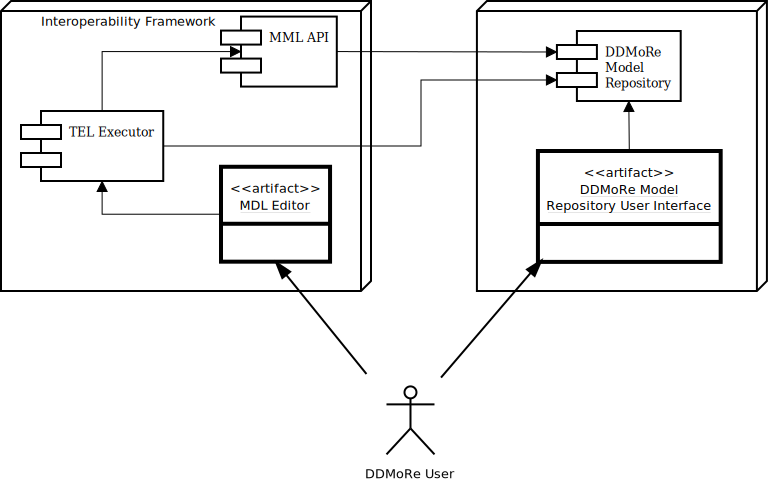
\includegraphics[width=0.75\linewidth]{img/UserInteraction}
	\caption{Overview of the interaction between \ddmore users and the Model Repository.}
	\label{fig:userInteraction1}
\end{figure}
\end{landscape}
\clearpage

\subsection{UML Activity Diagrams}
\label{appendix2}
\clearpage

\clearpage
%% Display the full name of authors and sort by author
\bibliographystyle{unsrt}
\bibliography{technical-specification}
\end{document}


%% Change the style of the glossary terms
\renewcommand{\glsnamefont}[1]{\textit{#1}}

\newcommand{\ddmore}{DDMoRe\xspace}

\newcommand{\idea}[1]{\fbox{\parbox{\linewidth}{\emph{#1}}}}
\makeglossaries

\begin{document}
%------------------------------------------------------------------------------
%Description       : DDMoRe WP7.2.1 Functional Specification for the Model
%                                   Repository Infrastructure - title 
%Author            : Mihai Glonț <mglont@ebi.ac.uk>
%Organization      : EMBL-EBI
%                    Wellcome Trust Genome Campus
%                    Hinxton
%                    Cambridge
%                    United Kingdom
%------------------------------------------------------------------------------
%% Don't insert a break after the title page.
\let\endtitlepage\relax

\fancypagestyle{firstpage}
{
    \fancyhf{}
    \fancyhead[R]{
\includegraphics[scale=0.5]{img/ddmore_logo}}
}

\begin{titlepage}
\thispagestyle{firstpage}
\begin{center}
{\huge Functional Specification of the \ddmore Repository Infrastructure}\\[15pt]

{\LARGE WP7 Sub-Task 7.2.1}\\[10pt]

Camille Laibe
\qquad Mihai Glon\textcommabelow{t}
\\[5pt]

\textsc{{\footnotesize EMBL-EBI, Wellcome Trust Genome Campus, Cambridge, United Kingdom}}
\end{center}
\end{titlepage}

\section*{Document Revision History}
\begin{tabularx}{\linewidth}{| c c X |}\hline
\textit{Date} & \textit{Author} & \textit{Comments} \\ \hline
1 August & Mihai Glon\cb{t} & First draft \\ \hline
\end{tabularx}

\section*{Copyright Notice}
Copies of this document may be distributed to any person within the Drug Disease Model Resources(\ddmore) project either in print or electronically, provided that they contain this Copyright Notice. 

%------------------------------------------------------------------------------
%Description       : DDMoRe WP7.2.1 First Technical Specification for the Model
%                                   Repository Infrastructure - Abstract 
%Authors           : Mihai Glonț <mglont@ebi.ac.uk>
%                    Camille Laibe <laibe@ebi.ac.uk>
%Organization      : EMBL-EBI
%                    Wellcome Trust Genome Campus
%                    Hinxton
%                    Cambridge
%                    United Kingdom
%------------------------------------------------------------------------------
\section*{Abstract}
\label{abstract}
This document describes the infrastructure required by the \ddmore Model Repository. It reviews the high-level architecture of the Repository in relation to the wider context of the project, outlining along the way design recommendations, flow of control, wire-frame mock-ups as well as potential software dependencies of the Repository.

The intended audience for this technical specification are the EFPIA and academic partners that are interested in the implementation of an instance of the Repository, as well as stakeholders that wish to interact, at a software level, with the Repository in an optimal manner.


\section*{Note on Requirement Levels}
The key words "MUST", "MUST NOT", "REQUIRED", "SHALL", "SHALL NOT", "SHOULD", "SHOULD NOT", "RECOMMENDED",  "MAY", and "OPTIONAL" in this document are to be interpreted as described in RFC 2119\cite{RFC2119}.

\section*{Convention}
Note that, for clarity, throughout this document the term \emph{Model Repository} is preferred over \emph{Model Library} and is used to denote the technical infrastructure required to store model descriptions along with code, data, algorithms, metadata, assumptions, Bayesian priors and links to references.
\clearpage
\setcounter{page}{1}
\tableofcontents
\listoffigures
\clearpage

\printglossaries
\clearpage

%% Each file contains a separate section to aid collaboration.
%------------------------------------------------------------------------------
%Description       : DDMoRe WP7.2.1 First Technical Specification for the Model
%                                   Repository Infrastructure - Introduction 
%Authors           : Mihai Glonț <mglont@ebi.ac.uk>
%                    Camille Laibe <laibe@ebi.ac.uk>
%Organization      : EMBL-EBI
%                    Wellcome Trust Genome Campus
%                    Hinxton
%                    Cambridge
%                    United Kingdom
%------------------------------------------------------------------------------
\section{Introduction}
\label{introduction}
This document provides a detailed description of the functionality that will be provided by the \ddmore Model Repository. The guidelines herein apply not only to the public Repository, but also to any private instances of it.

\subsection{Scope}
This document reviews the characteristics of the \ddmore Model Repository in relation to the wider context of the project, outlining along the way envisaged workflows, interactions with both users and third party software, as well as potential software dependencies of the Repository. The intended audience for this specification are the EFPIA and academic partners that wish to use the Repository in an optimal manner, or are merely interested in its capabilities.

\subsection{Non-Goals}
Although this task should deliver a technical specification at this stage according to the Description of Work, it is paramount that the behaviour of the Repository meets the needs of its end-users. Therefore, this document aims to offer a mental picture of the features that have been incorporated into the design of the Repository, allowing the interested stakeholders to flag up any shortcomings. Implementation-specific details about the inner-workings of the Repository are outside of the scope of this document, but will be discussed in the second technical specification which is due in month 42 of the project. 

\subsection{Context}
\label{context}
In a world where inefficient data and knowledge-sharing between academia, pharmaceutical companies and regulatory bodies hinders the development of better medicines, the Drug Disease Model Resources project (\ddmore) -- a Europe-wide effort funded by Innovative Medicines Initiative Joint Undertaking -- seeks to create an environment governed by standards that addresses these shortcomings. Specifically, the \ddmore consortium is developing a common definition language for data, models and work flows, as well as a standard for storing and exchanging \glspl{model} and associated \gls{metadata}\cite{ddmore:dow}.

The main focus on this specification is the objective of Task 7.2: the \ddmore Model Repository. It aims to provide a central repository for the models created by the project, encouraging their reuse. The Repository is closely linked with other deliverables of \ddmore. For instance, the pre-competitive models that will populate the Model Repository initially will be provided by Work Package 1. The models will be encoded in the XML-based format developed by WP4, and the Repository will rely on the software library created by Task 2.3 in order to manipulate the models. Finally, the published models stored in the \ddmore Model Repository will be showcased in the public instance of the Modelling Framework, generated by Task 7.1.

\subsection{Objectives}
\label{objectives}
The main objectives of the Repository are to provide:
\begin{itemize}
  \item a central, versioned, storage place for public and private models
  \item a way to display individual models
  \item a way to search for models
  \item a way to download models
  \item various means to access the stored \glspl{model}, making available the information encoded in MML to both users and tools. 
\end{itemize}

\subsection{Type of users}
\label{users}
This section classifies the users of the \ddmore Model Repository into categories. With the exception of Administrators, whose permissions are granted at global level, over the entire instance of the Repository, all other roles that require authentication are defined at the level of a specific revision. This means that the owner of one model can also be the editor of a revision for another model. 

\begin{description}
  \item[Visitor] an anonymous user accessing \glspl{published model}.
  \item[Owner] the user who submitted the model and has ultimate ownership of what is done to it and how and
when it is published.
  \item[Editor] any user who is able to modify and add information to an existing published or \gls{unpublished model}. Typically the Owner of a model is also an Editor of this model.
  \item[Collaborator] any user who is able to access an unpublished model.
  \item[Reviewer] a user who can access an unpublished model. This role can be limited in time.
  \item[Administrator] a user who is responsible for the security, management and maintenance of the system.
\end{description}

The interactions between users, the Model Repository and other components of the project (such as the Interoperability Framework) are depicted in Figure~\ref{fig:userInteraction}. As such, one may access the Repository directly -- through the web-based user interface -- or indirectly, via the Modelling Interoperability Framework, that uses the Task Execution Language (TEL) and the software library created in WP2.3 to access and store models in the \ddmore Model Repository.

\begin{figure}[htb]
\centering
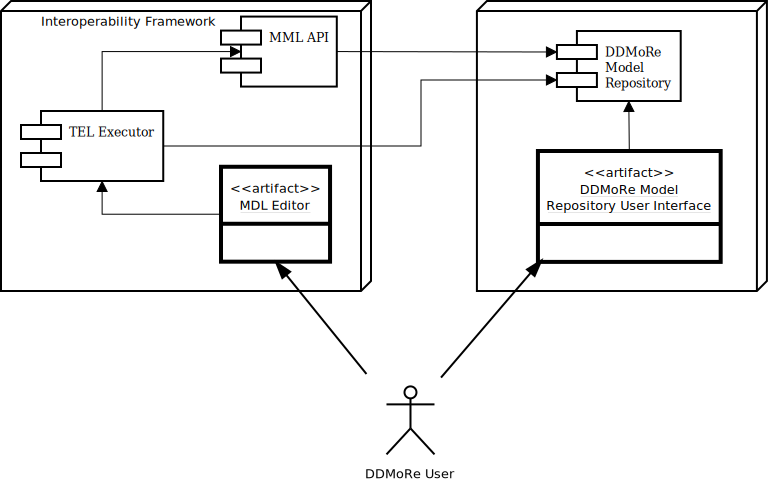
\includegraphics{img/UserInteraction}
\caption{Interactions between users, the interoperability framework and the Model Repository.}
\label{fig:userInteraction}
\end{figure}


%------------------------------------------------------------------------------
%Description       : DDMoRe WP7.2.1 First Technical Specification for the Model
%                                   Repository Infrastructure - Requirements Survey 
%Author            : Mihai Glonț <mglont@ebi.ac.uk>
%Organization      : EMBL-EBI
%                    Wellcome Trust Genome Campus
%                    Hinxton
%                    Cambridge
%                    United Kingdom
%------------------------------------------------------------------------------
\section{Requirements Survey}
\label{requirementsSurvey}
This section reviews the needs, goals and constraints of the \ddmore Model Repository. These requirements are divided in two categories: \textit{functional} - that is, relating to what the \gls{system} does, and \textit{non-functional}, describing the quality criteria that will be used to assess the system. The former are presented in Section~\ref{functionalRequirements}, while the latter are the subject of Section~\ref{nonFunctionalRequirements}.

\subsection{Functional Requirements}
\label{functionalRequirements}
%% Create a row counter so that we don't have to keep track of the ID of the functional requirement http://tex.stackexchange.com/questions/21243/automatic-table-row-numbers/21244#21244
%\newcounter{frCounter}
%\newcommand\frIndex{\stepcounter{frCounter}\arabic{frCounter}}

\begin{enumerate}[1]
\subsubsection{Model Management}
\item The system is REQUIRED to store models encoded in MML. 

\item The system MUST allow appropriate users to revise models encoded in MML. 

\item The system MUST allow specific revisions to be deleted by their owners, but no revision SHALL be lost from the Repository. Consequently, users that had access to a model revision before its deletion SHALL continue to do so. The system SHOULD inform the user about the removal and MAY supply a link to a model revision which replaces it, if this information has been specified by the user that performed the deletion. 

\item The system MUST enable the creation of new MML models based on either an existing one, or a template. The system SHALL record for the new model a reference  to the representation from which it derives.

\item The system is REQUIRED to ensure that model representations are faithful to the MML specification either on-demand -- upon request, or autonomously -- whenever the need arises, such as before accepting a new revision for a model. 

\item Functionality equivalent to a software version control system is REQUIRED. All changes to the MML MUST be preserved and be accessible. In particular, the system SHALL ensure that concurrent modifications of models are dealt with appropriately.

\item Programmatic access to and manipulation of models within the Repository MUST be provided to other software systems including, but not limited to those within \ddmore. 

\item Users MAY be able to inspect differences between different versions of the same model.

\item The system MAY enable MML model representations contained within it to be developed via an integrated text editor.

\subsubsection{Model Browsing, Searching and Retrieving}
\item The system MUST be able to search the latest revision of model descriptions based on a textual term such as name, author, date of creation, date of modification, or any other textual field in MML. The results SHOULD only include models to which the user has access to.

\item The system MUST allow a selection of search results, bundled as an archive, to be downloaded.

\item Models MUST be displayed in an organised and user-friendly manner.

\item Users SHALL be able to retrieve and download any revision of any model they can access.

\item Model annotation data SHOULD be included in the model search.

\item The system SHOULD be able to search for models based on complex queries, with ranked results.

\subsubsection{Authentication and Authorisation}
\item The system MUST authenticate users and ensure that they can only perform the role assigned to them for a given model (cf. section~\ref{stakeholders}).

\item In order to allow the creation of an audit trail, each revision MUST be stored with metadata such as the identity of the user performing the action and a timestamp. The granularity of the audit trail SHOULD be configurable at the level of the instance by an Administrator. Users MAY add a comment describing the changes.

\item A model owner MUST be allowed to grant read and write access to a model using one of the following options:
\begin{inparaenum}
\item a single revision 
\item all existing revisions 
\item all revisions including the ones in the future. 
\end{inparaenum} 

\item Once granted, read rights to a revision for a particular user SHALL NOT revoked, the reason being that once a user has gained read access to a model, they might have already collected all relevant information.

\item The system MUST enable users to revoke write access to future revisions of a model for a single user or multiple users simultaneously.

\item The system MUST enable model owners to publish a single version of a model. This action SHALL not impact the status of previous model revisions. 

\item The Owner SHOULD be able to grant write access to a model to a single user, or to a group of users. This would allow collaborators to upload new model revisions. The system is then REQUIRED to automatically grant read and write access to a revision for the collaborator that uploads it.

\item A model owner SHOULD be allowed to transfer the complete ownership of a model to another user of the system.

\item The owner SHOULD be able to control the access rights of other users to read or write the model, according to the roles defined in section~\ref{stakeholders}.

\item The level of visibility of the audit information associated with a published model SHOULD be configurable at the level of the instance by an Administrator.

\item Unauthenticated access to the published models in the system SHOULD be permitted as a configuration option. If this option is disabled, users MUST be authenticated before they can access any models within the system.

\item The system MUST be protected against SQL injection, cross-site scripting as well as cross-site request forgery attacks. 

\subsubsection{Technology}
\item The system SHALL store models represented in MML format.

\item The server side of the system is REQUIRED to work on a Linux platform with Kernel version~$\ge 2.6$. 

\item The client side SHALL work with the following operating systems: Mac OS X (All platforms down to Leopard, Version 10.5.x), Windows (All platforms down to Windows XP), Linux (Kernel version~$\ge 2.6$).

\item The client side MUST work with the following web browsers: Safari Version 5.x and above, Internet Explorer 8 and above, Firefox Version 6.x and above. The front end MAY work in other browsers, but full compliance is only required for the internet browsers listed above.

\item An established software version control system such as Subversion, Mercurial or Git MAY be used by the system internally, however, it MUST NOT be exposed to users directly.

%% user management requirements are missing from the original document
\subsubsection{ User Management}
\item An administrator MUST be able to manage accounts. This covers creation, suspension, deletion, blocking or unblocking.

\item The system MUST allow an authenticated user or administrator to update certain details of an account including but not limited to password, or real name of the user. Due care MUST be taken to ensure that the user confirms their identity before editing this information.
\end{enumerate}

\subsection{Non-functional Requirements}
\label{nonFunctionalRequirements}
\begin{enumerate}[1]
\setcounter{enumi}{50}
\item The system MUST be responsive, completing 80\% of requests in under 10 seconds and 95\% of requests in under 30 seconds on a computer with 2GB RAM, dual-core processor and 1Mb/s Internet connection.

\item The user interface of the system  SHALL be designed with usability in mind, displaying information in a meaningful and user-friendly manner to its stakeholders, without overloading them.

\item The system MUST NOT crash.

\item The look and feel of the Repository MUST be configurable by means of instance settings.

\item The system SHALL notify users when a request cannot be processed immediately and indicate the progress.

\item The system SHALL be implemented using modern presentation and accessibility standards in order to aid maintainability.

\item The system SHOULD be installable and configurable as a software distribution.

\item The system SHOULD be modular and permit extension.
\end{enumerate}


%------------------------------------------------------------------------------
%Description       : DDMoRe WP7.2.1 First Technical Specification for the Model
%                                   Repository Infrastructure - Proposed Design 
%Author            : Mihai Glonț <mglont@ebi.ac.uk>
%Organization      : EMBL-EBI
%                    Wellcome Trust Genome Campus
%                    Hinxton
%                    Cambridge
%                    United Kingdom
%------------------------------------------------------------------------------
\section{Proposed Design}
\label{proposedDesign}
\idea{Add general description of the topics covered in this section.}

\subsection{Stakeholders}
\label{stakeholders}
This section classifies the users of the \ddmore Model Repository into categories. With the exception of Administrators, whose permissions are granted at global level, over the entire instance of the Repository, all other roles that require authentication are defined at the level of a specific revision. This means that the owner of one model can also be the editor of a revision for another model. 

%\idea{Description of the types of users that will use the Repository.}

\subsection{Use Cases}
\label{useCases}
The aim of this section is to describe how each of the aforementioned stakeholders interact with the system. Each such interaction is called a \emph{use case}, while the user performing it is known as an \emph{actor}. The use cases listed in Figure~\ref{fig:useCases} only consider the main actors that are involved, hence Administrators are not mentioned in any model-related use cases, in spite of the fact that they do have the authority required to perform any action. 

\begin{figure}[htb]
\centering
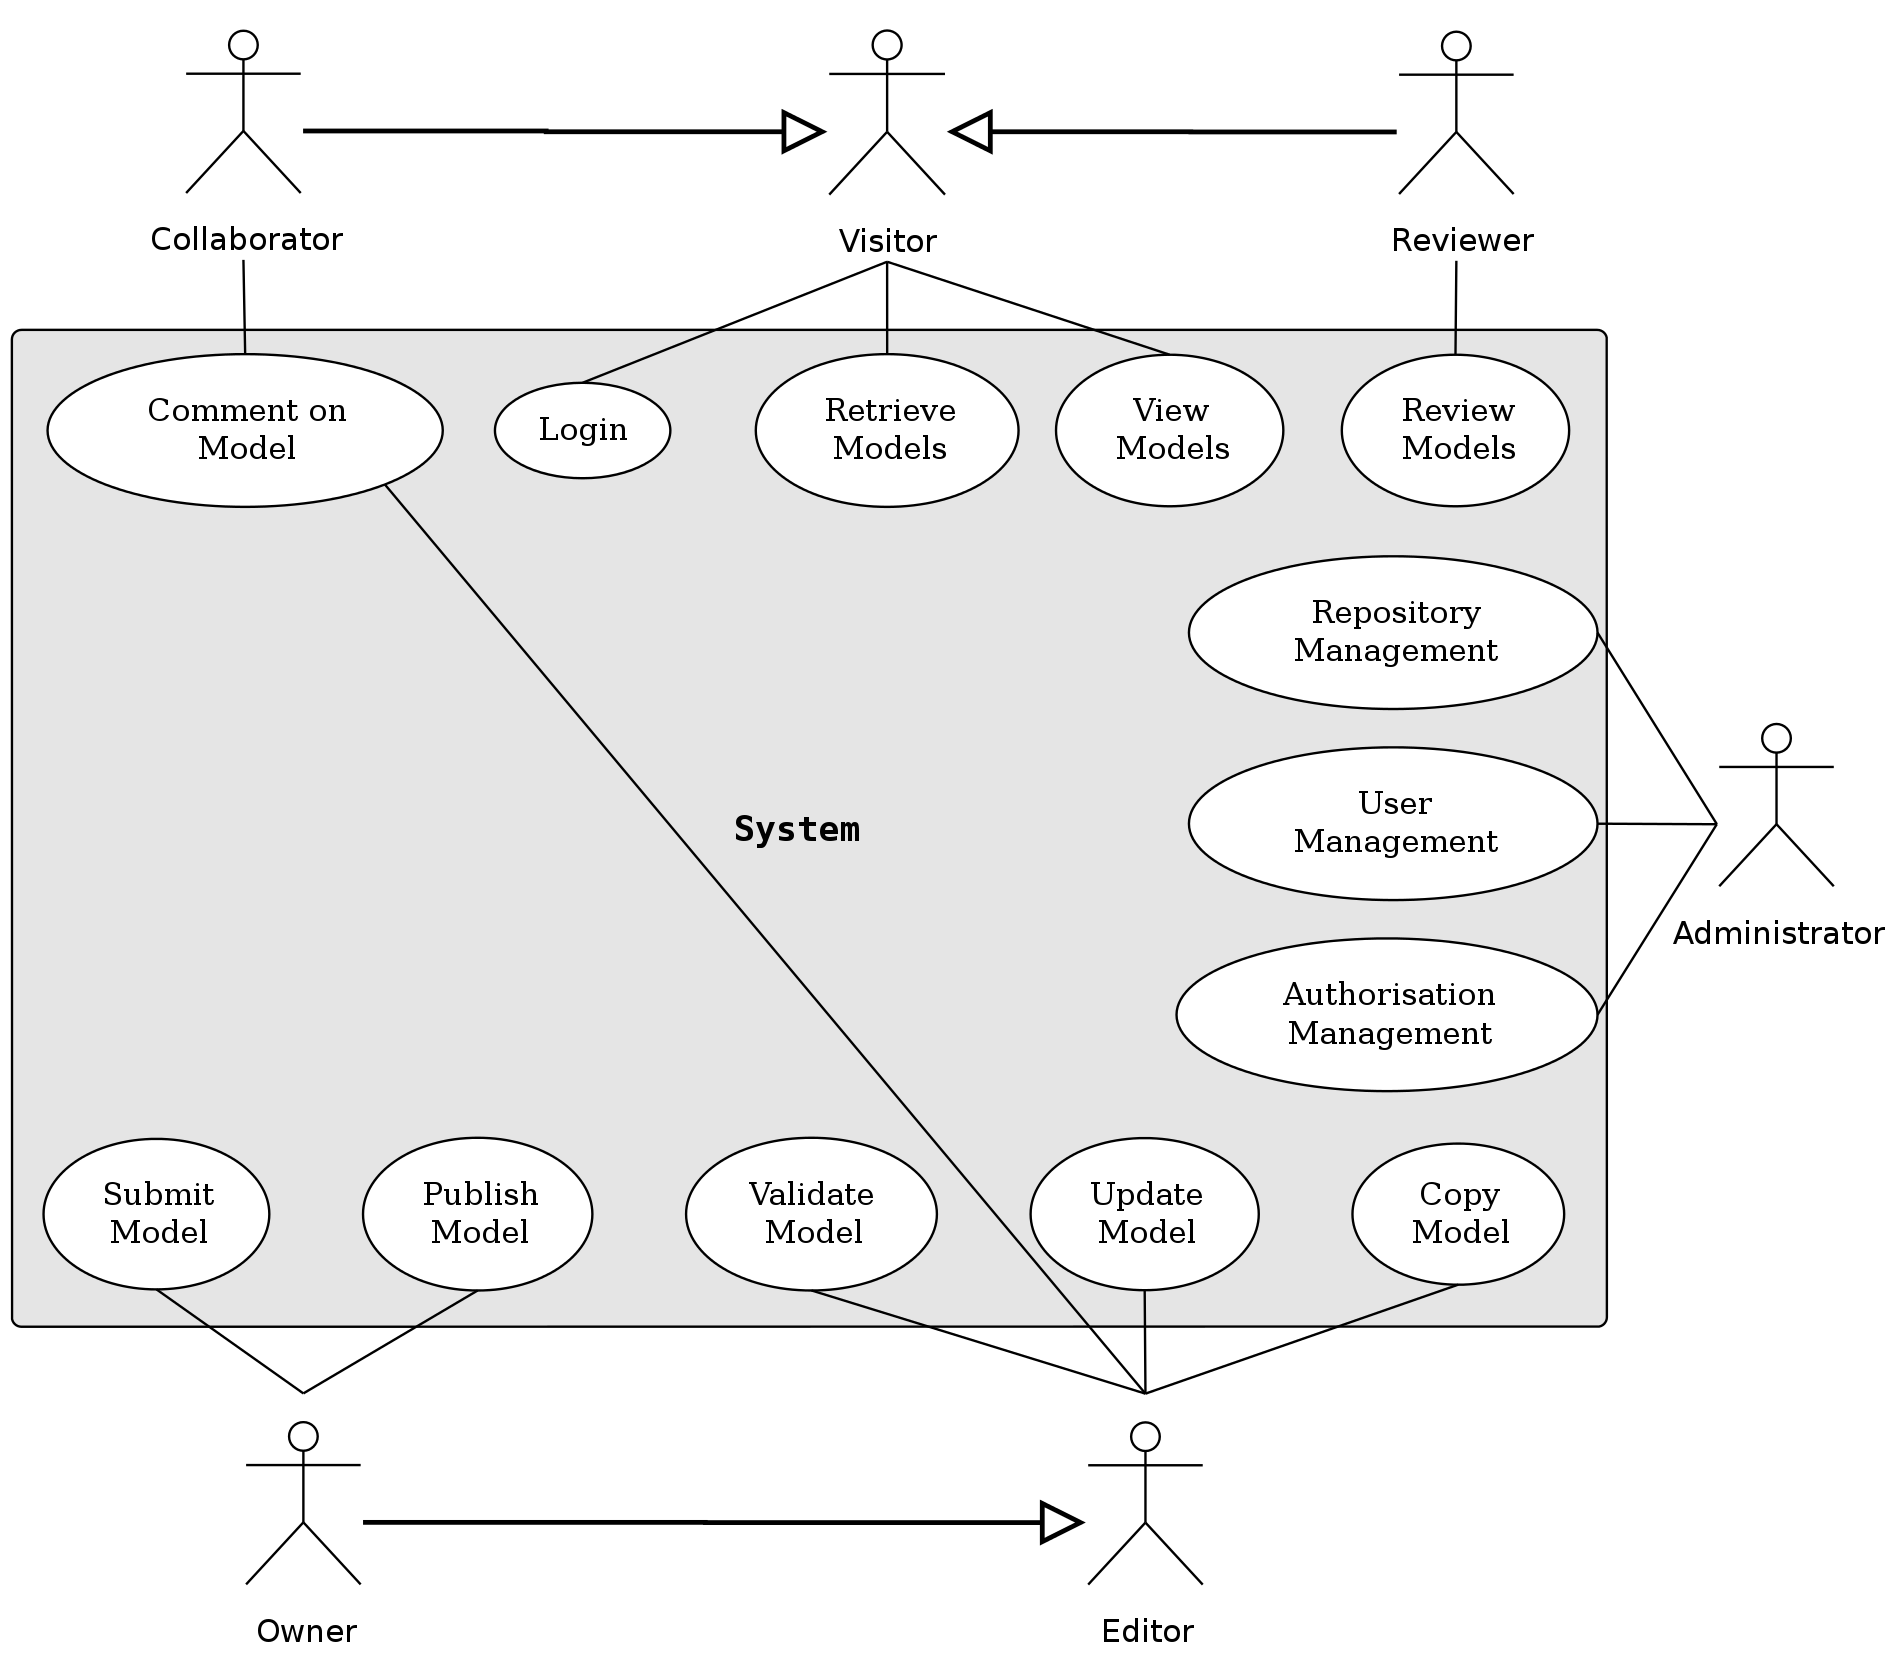
\includegraphics[scale=0.33]{img/UseCases}
\caption{Diagrammatic representation of the system's scope.}
\label{fig:useCases}
\end{figure}

\subsection{Proposed Work flows}
\label{workFlows}
\idea{UML Activity and Sequence diagrams should go in the appendix, should there be many of them. This section should only discuss them.} 

\subsection{Software Infrastructure}
\label{softwareInfrastructure}
\idea{Add UML Deployment diagram showing the link between a DB server, a Web server (possibly a servlet container behind an HTTP server) and a folder under version control.}

\subsection{Mock-ups}
\label{mockUps}
\idea{General UXD comments behind the look and feel of the pages. Actual mock-ups should be in the appendix. Landscape page format might be required for this part.}

%------------------------------------------------------------------------------
%Description       : DDMoRe WP7.2.1 First Technical Specification for the Model
%                                   Repository Infrastructure - Web Services
%Author            : Mihai Glonț <mglont@ebi.ac.uk>
%Organization      : EMBL-EBI
%                    Wellcome Trust Genome Campus
%                    Hinxton
%                    Cambridge
%                    United Kingdom
%------------------------------------------------------------------------------
\subsection{Programmatic Interaction with the \ddmore Model Repository}
\label{webServices}
\idea{This section is dedicated to programmatic access to and manipulation of models. It should provide a diagrammatic representation of the envisaged architecture along with the considerations behind it. A discussion on the integration with other software systems within \ddmore should also be included.}



\subsection{Security Considerations}
\label{securityConsiderations}
\idea{Exclude data centre, hardware and network security aspects from the scope of this document. Recommend running the HTTP server and the servlet container as different users with limited privileges. Beware that the user running the servlet container needs write access to the folder storing models. Discuss the need to protect the metadata directory within the folder where the models are stored (e.g. .git, .hg, .svn), as access to them outside the designated protocol - i.e. the web interface - should be prohibited.}

\subsection{Licence}
\label{licence}
The code for the \ddmore Model Repository will be hosted on SourceForge and released under a GPL-compatible licence. This licence does not apply to the models stored in either the public Repository or any private instance of it. 


%\begin{landscape}
\section{Appendices}
\label{appendices}
\subsection{Mock-up Designs}
\label{appendix1}

\begin{figure}[htb]
	\centering
	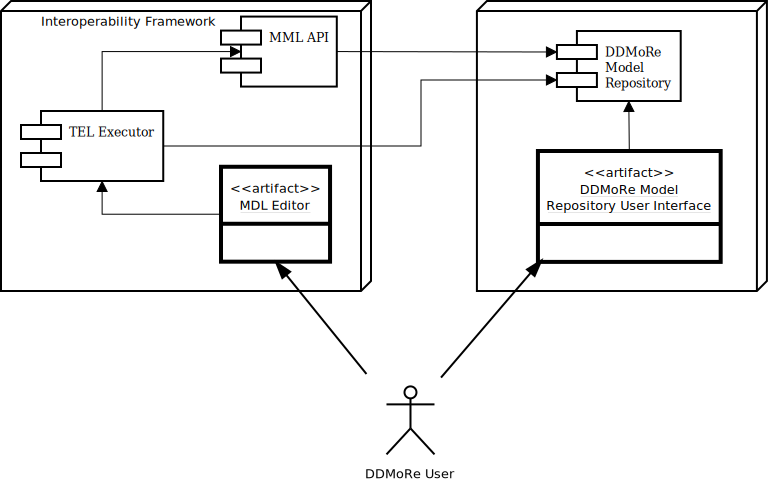
\includegraphics[width=0.75\linewidth]{img/UserInteraction}
	\caption{Overview of the interaction between \ddmore users and the Model Repository.}
	\label{fig:userInteraction1}
\end{figure}
\end{landscape}
\clearpage

\subsection{UML Activity Diagrams}
\label{appendix2}
\clearpage

\clearpage
%% Display the full name of authors and sort by author
\bibliographystyle{plain} 
\bibliography{technical-specification}
\end{document}
